\chapter{Testování aplikace}
Kapitola testování aplikace je rozdělena na dvě části. První část tvoří popis prostředí, které je potřebné pro spuštění aplikace. Druhá část testování je zaměřena na praktické testování fungování aplikace. 
\section{Definice prostředí pro testování aplikace}
Testovací prostředí je vytvořeno na linuxové distribuci Ubuntu. První částí, kterou je potřeba spustit je k8s API a Etcd databáze, které představují Customer API se kterým uživatelé přímo komunikují. Kubernetes komunita vytvořila kód, který umožňuje \linebreak spustit k8s cluster na lokálním počítači \cite{local-cluster}. Spuštění k8s clusteru lokálně závisí na technologiích Docker, Etcd a programovacím jazyce Golang, které musí být na lokálním stroji nainstalovány. Dále musí být nainstalovány nástroje pro práci s certifikáty OpenSSL a CSFSSL, které k8s vyžaduje pro své fungování. V dalším kroku je spuštěn bashový skript, který vytvoří ze zdrojových kódů binární soubory jednotlivých služeb k8s, které jsou následně spuštěny. Skript také vytvoří Kubeconfig soubor pro komunikaci s k8s API. Pro běh aplikace jsou potřebné pouze komponenty k8s API a databáze Etcd, ostatní komponenty jako jsou scheduler a controller-manager mohou být vypnuty.\par 
    Pro reprezentaci k8s clusteru je využita technologie Minikube. Minikube je nástroj, který umožňuje snadno, pomocí jednoho příkazu, spustit k8s cluster. Minikube je možné spustit na Windows, macOs nebo Linuxovém operačním systému. Minikube na lokálním počítači spustí virtuální server ve kterém je již k8s připravené na použití. Minikube cluster je plnohodnotný k8s cluster, který běží všechny služby v jednom virtuálním stroji. \par
\section{Testování distribuce Kubernetes objektů}
    Cílem testování je ověřit jak prototyp aplikace distribuuje zdroje z virtuálního clusteru do plnohodnotného k8s clusteru, který reprezentuje nástroj Minikube. Kubectl je nástroj příkazového řádku, který umožňuje vytvářet zdroje v k8s clusteru a vzdáleně tento cluster ovládat. Informace o jednotlivých clusterech jsou definovány v kubeconfig souborech. Kubectl nástroj dovoluje přepínat mezi jednotlivými kubeconfig soubory (kubectl používá kontexty pro rozlišení jednotlivých clusterů) a ovládat takto rozdílné k8s clustery. Pro snadnější přepínání mezi jednotlivými k8s clustery, je použit skript \ref{lst:script}, který umí přepínat mezi jednotlivými kontexty. Přepnutí kontextu se vykoná pomocí příkazu swc <název kontextu>.  
    
\begin{lstlisting}[caption={Bash skript pro práci s k8s kontexty},label=lst:script]
#!/bin/bash
if [ "$1" == "-h" ]; then
  echo "Usage: $0 [swc local - switch to local Kubernetes context]"
  exit 0
fi
if [ "$1" == "list" ]; then
  kubectl config get-contexts
  exit 0
fi

kubectl config use-context $1
\end{lstlisting}

    Pro lepší přehlednost ve kterém clusteru byl znázorněný příkaz vykonán je upraven terminál tak, že zobrazuje aktuální název clusteru. Na obrázku \ref{fig:prompt} první řádek zobrazuje local cluster, to znamená že současný kontext je nastaven na virtuální k8s api. Dále je na prvním řádku spuštěn příkaz, který zobrazí seznam dostupných kontextů, kde hvězdičkou je označený aktivní kontext. Poté následuje swc příkaz \ref{lst:script}, který přepne kontext na minikube cluster a změní se i popisek řádku, který říká že aktuální kontext je minikube.\par

\begin{figure}[H]
  \begin{centering}
    
	  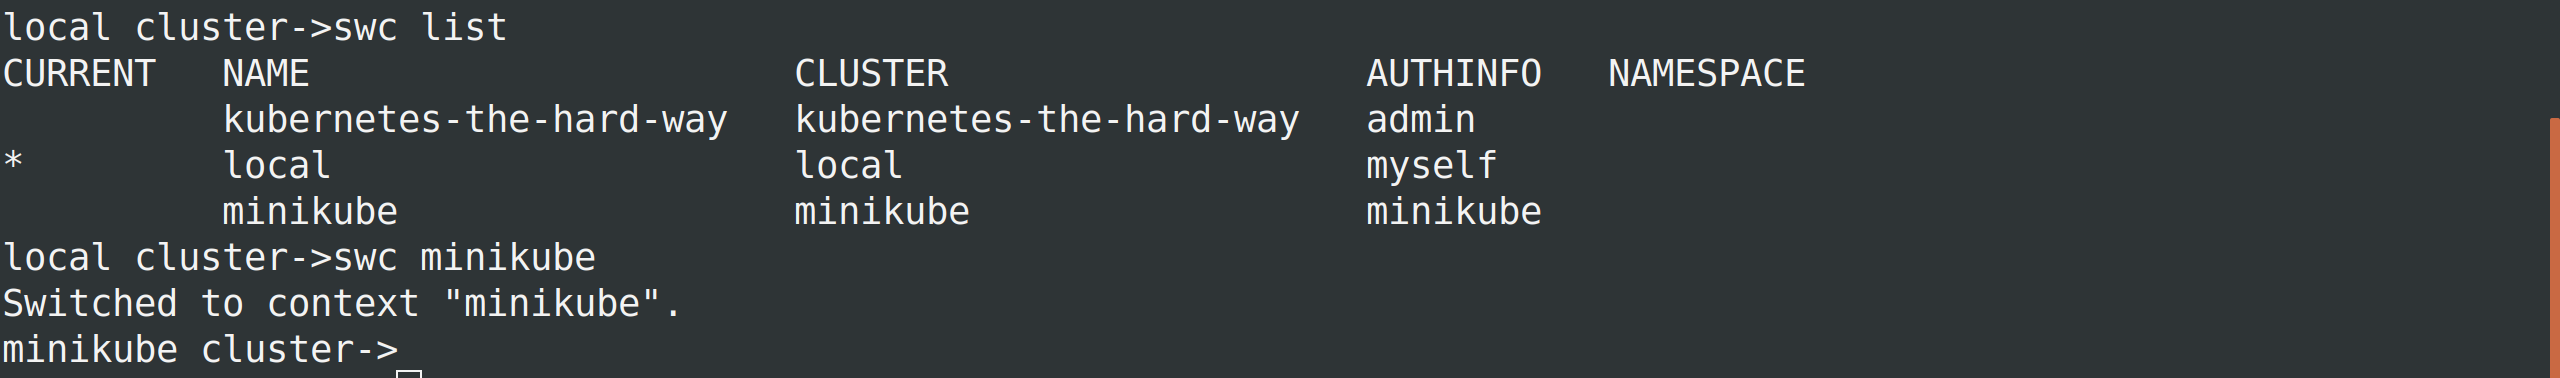
\includegraphics[width=0.9\textwidth]{images/prompt.png}
    \par
	  \caption{Vzhled terminálu\label{fig:prompt}, zdroj: vlastní tvorba}
    \end{centering}
\end{figure}

\subsection{Distribuce Kubernetes node objektů}
    Aplikace umožňuje uživatelům sledovat jednotlivé zdroje a to i servery, které provozují jejich aplikace. V k8s jsou tyto servery označeny jako nody. Na obrázku \ref{fig:nodes-init} je zobrazen seznam dostupných nodů. První je lokální cluster, který reprezentuje virtuální k8s API a obsahuje jeden node s verzí 1.15.0-alpha a dalšími parametry. Druhý cluster minikube obsahuje rovněž jeden node, ovšem s rozdílnými parametry, např. jméno, role nebo verze.\par

\begin{figure}[H]
  \begin{centering}
    
	  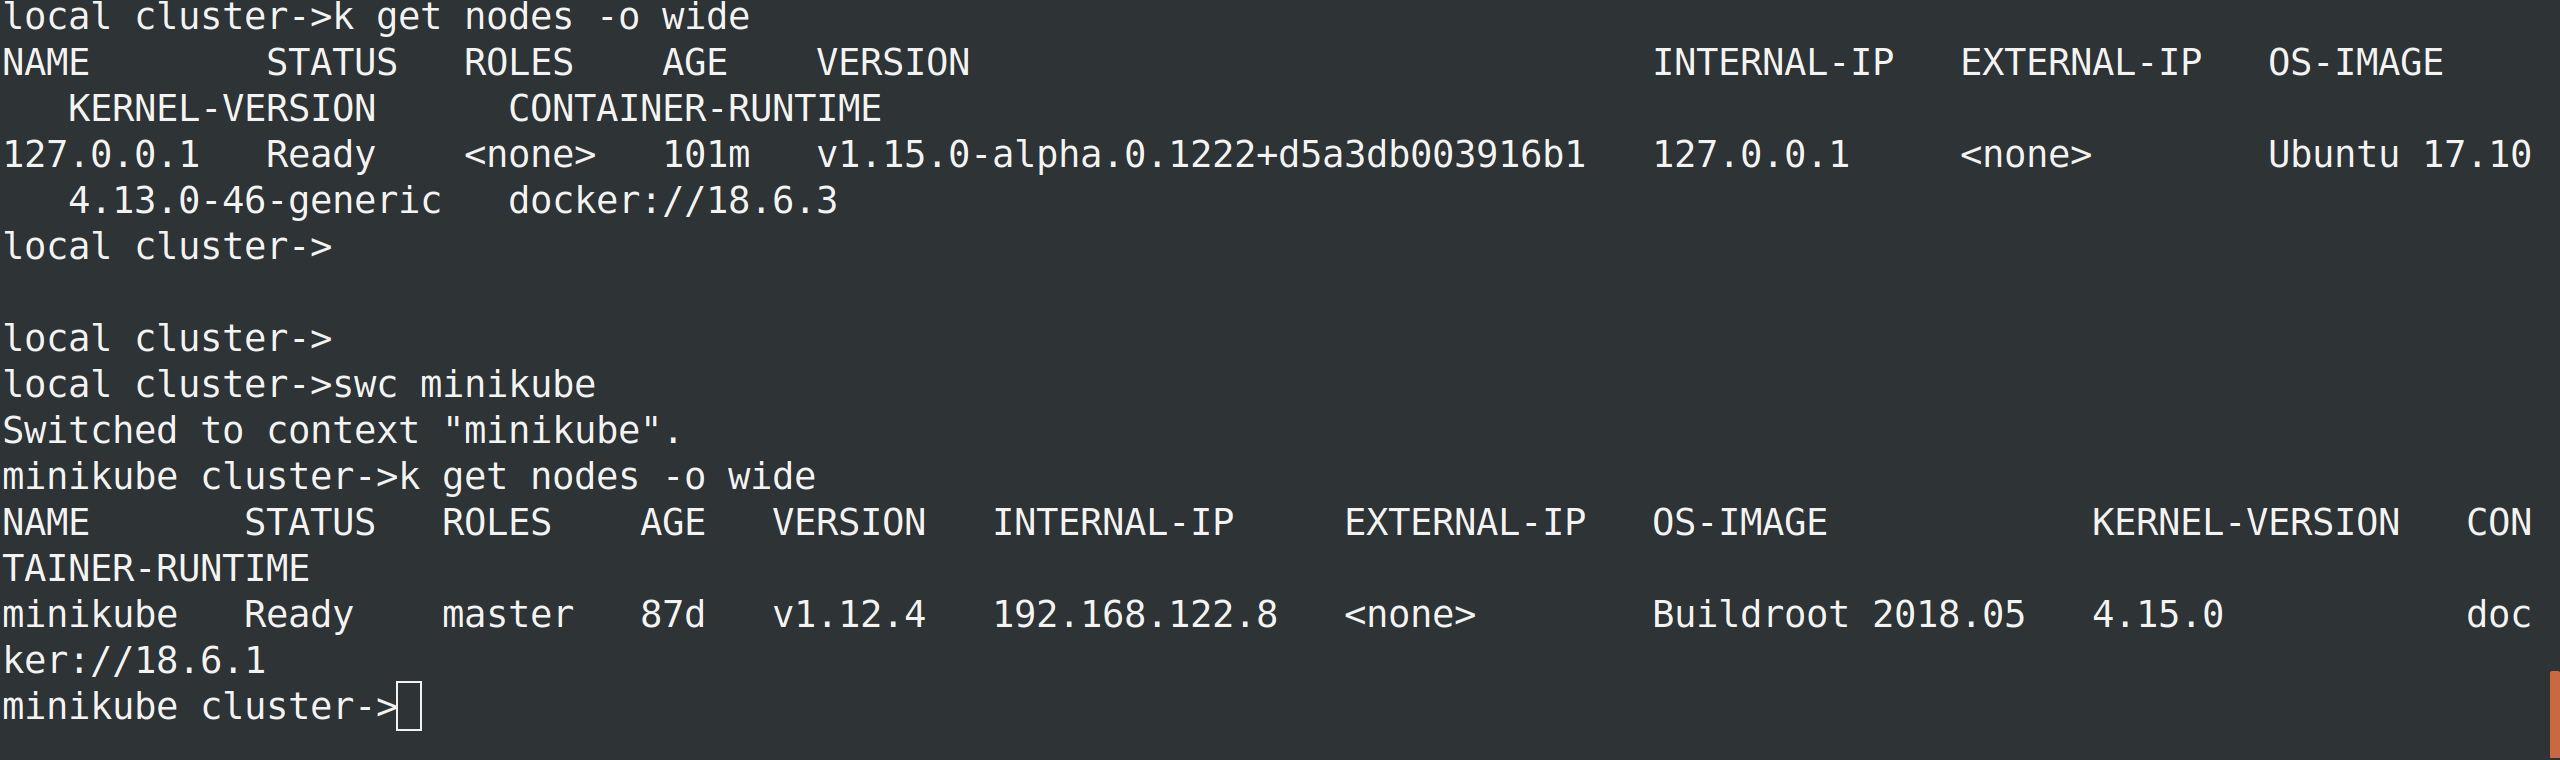
\includegraphics[width=0.9\textwidth]{images/nodes-init.png}
    \par
	  \caption{Seznam nodů v jednotlivých clusterech\label{fig:nodes-init}, zdroj: vlastní tvorba}
    \end{centering}
\end{figure}

    Po spuštění aplikace dojde k inicializace a spuštění managerů. Minikube manager informuje customer manager o dostupných zdrojích. V současné chvíli zde nejsou vytvořeny žádné zdroje. Minikube manager tak oznámí customer manageru informace o nodech, které má zaregistrované. Customer manager tuto událost obdrží a uloží tyto informace do virtuálního k8s API, kde si je uživatelé mohou prohlédnou. Výsledek této akce je uveden na obrázku \ref{fig:nodes-initialized}. Uživateli jsou zobrazeny nody v obou clusterech společně s jejich vlastnostmi.


\begin{figure}[H]
  \begin{centering}
    
	  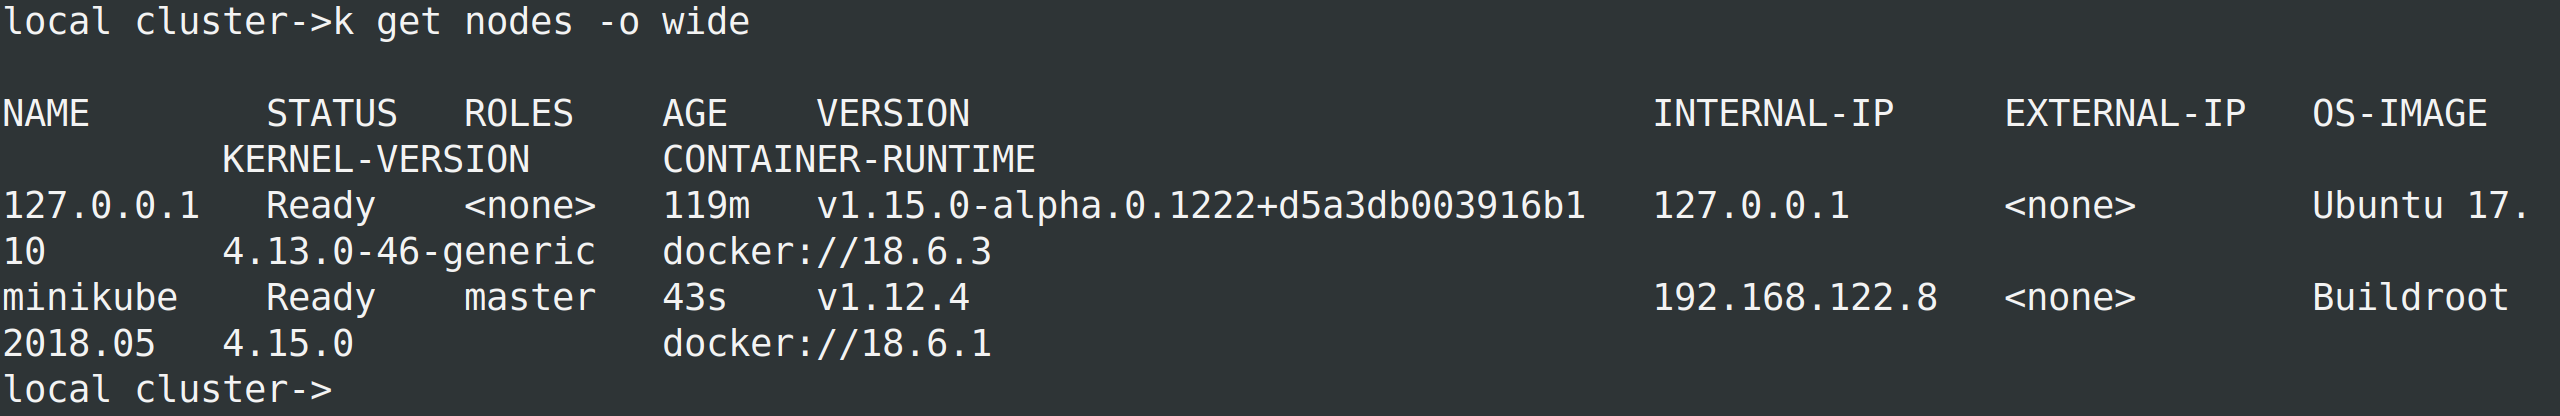
\includegraphics[width=0.9\textwidth]{images/nodes-initialized.png}
    \par
	  \caption{Seznam nodů po spuštění programu\label{fig:nodes-initialized}, zdroj: vlastní tvorba}
    \end{centering}
\end{figure}

\subsection{Distribuce Kubernetes pod objektů}
    Dalším testovaným scénářem je testování distribuce podu z centrálního API do \linebreak Minikube clusteru. Spouštění podů je základní a nezbytná funkce k8s clusterů. Nástroj kubectl umí vytvářet zdroje, které jsou definované s souborech, nazývaných manifesty. Definice podu je uvedena na ukázce kódu \ref{lst:pod}. Definice podu začíná parametrem apiVersion, který specifikuje verzi API, která bude použita pro vytvoření objektu. Parametr Kind uvádí typ objektu, v tomto případě se jedná o pod. Další částí jsou metadata, která připojují další informace o objektu jako jsou jméno nebo id objektu, případně namespace ve kterém má být objekt vytvořen. Posledním blokem jsou spec informace. Zde se nachází definice kontejneru, případně více kontejnerů, který má být v podu spuštěný. Nejdříve je nastaveno, že k8s nemá restartovat kontejner, dále název kontejneru uvnitř podu a definice kontejneru s aplikací. Konkrétně bude spuštěn kontejner BusyBox. Jedná se o malou linuxovou distribuci, která poskytuje základní nástroje pro práci se systémem. Po spuštění kontejneru bude vypsána hláška a dojde k ukončení kontejneru.
\begin{lstlisting}[caption={pod.yml, definice podu},label=lst:pod]
apiVersion: v1
kind: Pod
metadata:
  name: test-pod
  labels:
    app: testapp
spec:
  restartPolicy: Never
  containers:
  - name: test-container
    image: busybox
    command: ['sh', '-c', 'echo Hello world !']
\end{lstlisting}
			  Proces vytvoření zdroje pod je uvedena na obrazku \ref{fig:pod}. Po aplikovaní manifest souboru je spuštěn proces vytvoření zdroje. Customer manager zjistí vytvoření zdroje pod a vytvoří událost s odpovídajícími parametry, kterou odešle do minikube manageu. Ten vytvoří pod v minikube clusteru a o jeho stavu informuje customer manager. Pod se nejdříve nachází ve stavu Pending, během něhož je určeno na kterém nodu bude spuštěn a také dochází ke stažení potřebného kontejner image. Poté je kontejner ve stavu Running, neboli vykonává zadaný kód, výpis hlášky. Po úspěšném dokončení výpisu přechází kontejner do stavu Completed. Stejný výstup vypíše i minikube cluster. Stav podu je shodný v obou clusterech.
			  Z minikube clusteru je možné vypsat průběh programu. Zde je vidět, že program vypsal hlášku “Hello world !”. Posledním krokem je odstranění podu. Zde bylo potřebné upravit kod aplikace, Aplikace totiž sleduje zdroje v určeném namespacu a aplikuje všechny informace o těchto zdrojích do minikube clusteru v případě customer managera. Na druhé straně minikube manager aplikuje všechny změny z minikube k8s clusteru do centrálního API s využitím customer managera. Při tomto nastavení docházelo k zacyklení aplikace. Zdroj byl sice smazán v centrálním API ale než tato informace doputovala do minikube clusteru, minikube manager oznámil centrálnímu API informace o běžícím podu. Jako řešení je použit postup v customer manageru, který ověří příchozí události z minikube managera a dovolí vytvořit pouze objekt Node. Vytvoření je reprezentováno jako parametr type s hodnotou Added struktury Event, která reprezentuje událost. 
			   
\begin{figure}[H]
  \begin{centering}
    
	  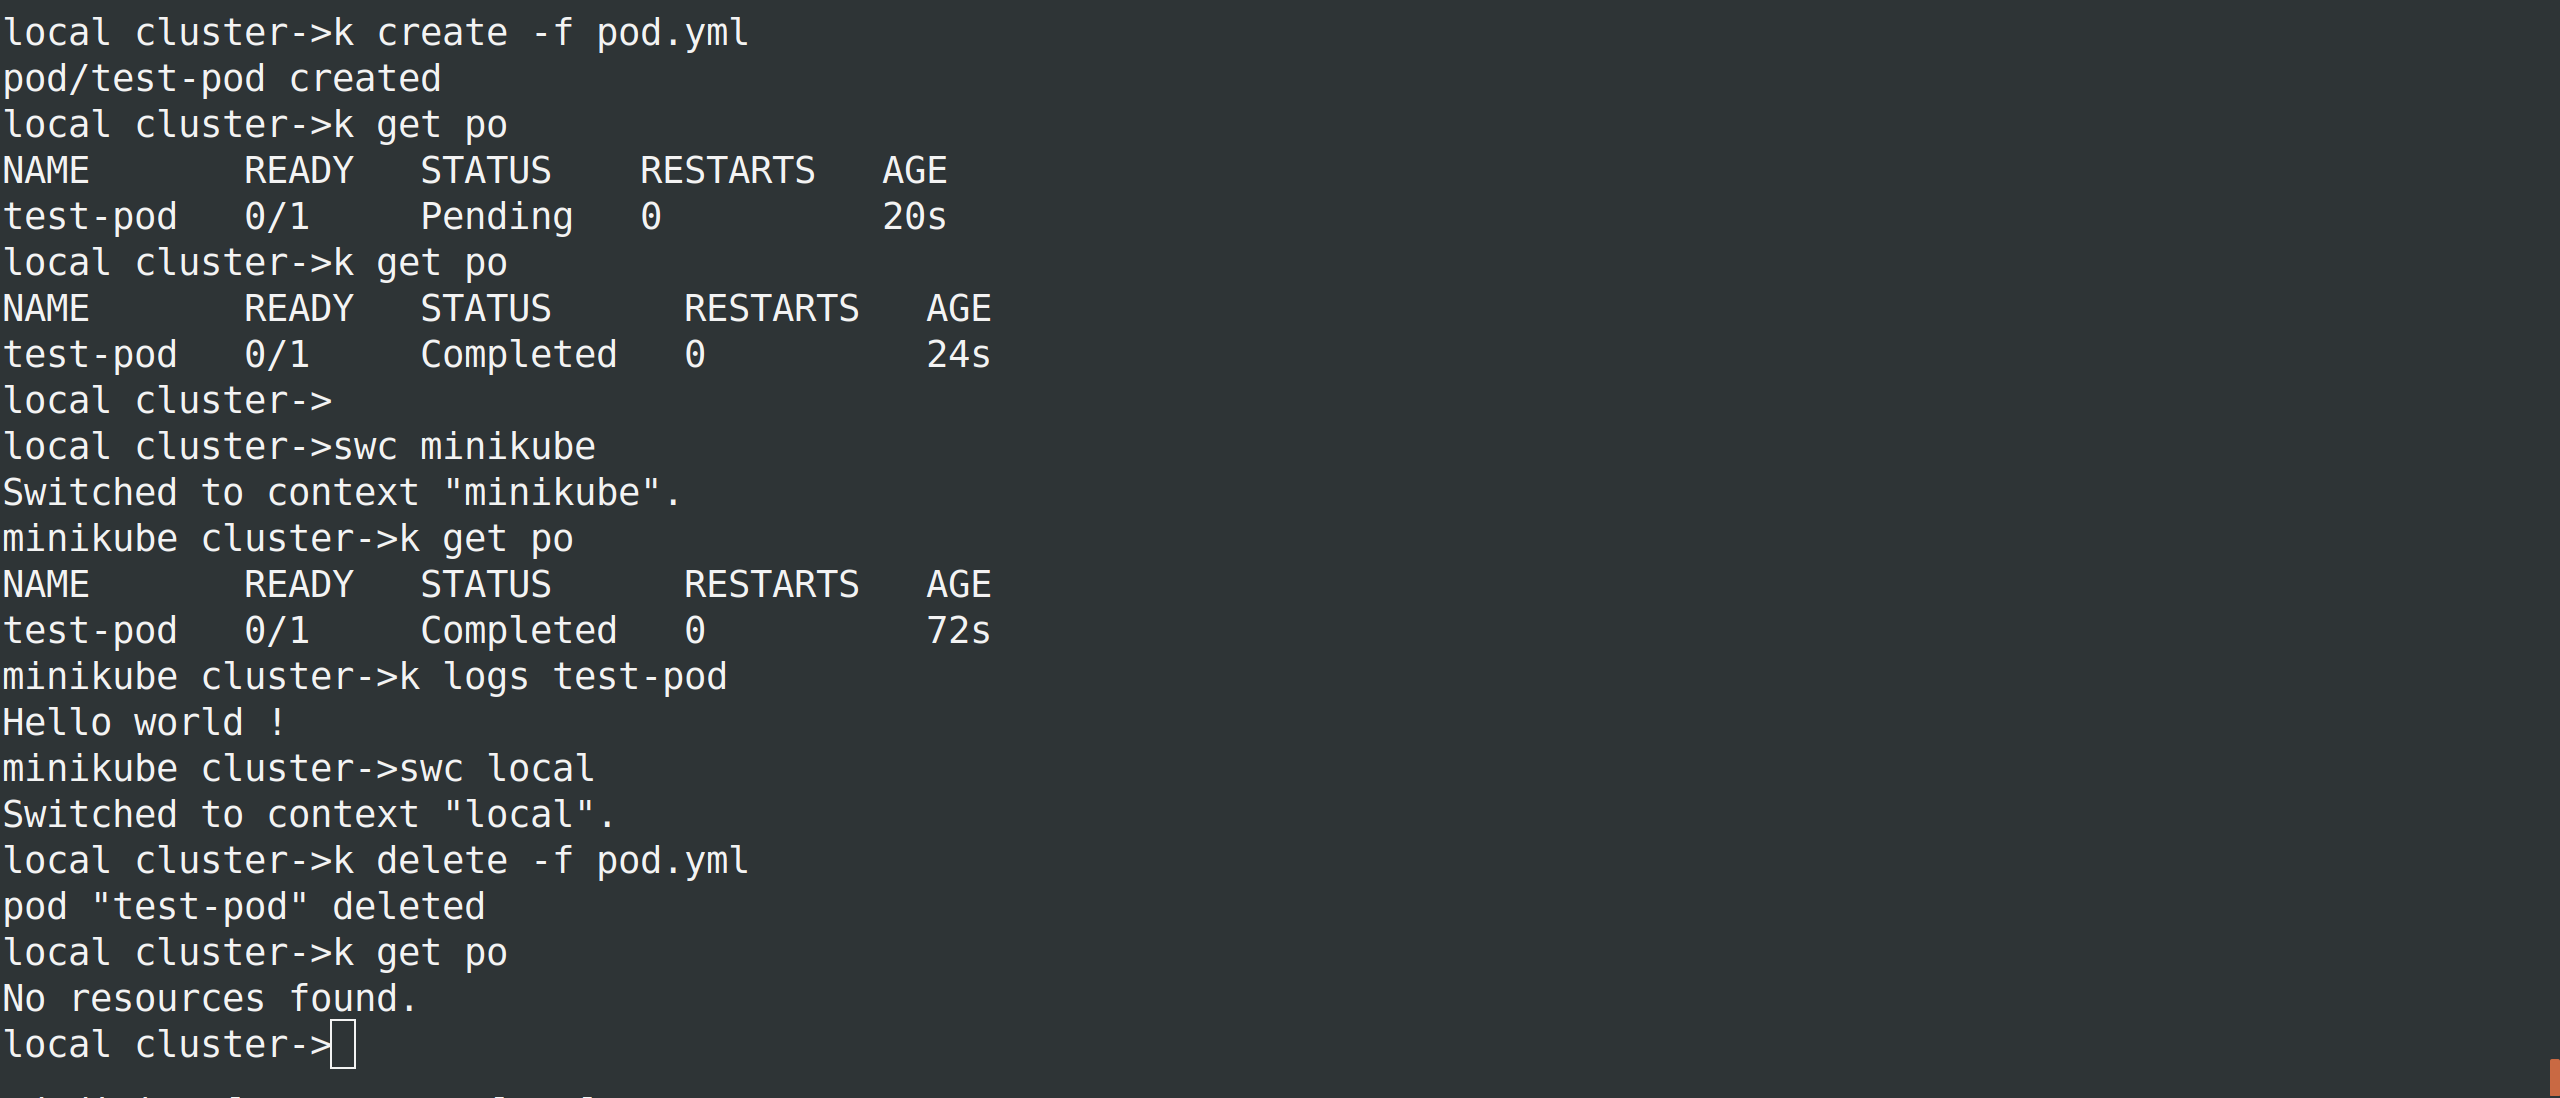
\includegraphics[width=0.9\textwidth]{images/pod.png}
    \par
	  \caption{Práce s pody\label{fig:pod}, zdroj: vlastní tvorba}
    \end{centering}
\end{figure}

\subsection{Distribuce Kubernetes deployment objektů}
Deploymenty řídí bezstavové, stateless, aplikace běžící v clusteru. Deployment umí udržovat potřebný počet kontejnerů, zvyšovat nebo snižovat počet kontejnerů, provádět přechod na novější verzi aplikace, případně vrátit původní verzi aplikace v případě, že nová verze obsahuje chyby. Definice deploymentu je uvedena na ukázce kódu \ref{lst:deployment}. V části spec je specifikován počet kontejnerů, neboli počet instancí aplikace. Další důležitou částí je selector, podle kterého jsou vybrány spravované kontejnery. Diky selectoru například udržuje deployment počet kontejnerů, pokud je počet kontejnerů s požadovaným labelem menší než je definováno, jsou vytvořeny nové kontejnery. V bloku template je definovaný kontejner a také jeho label a port na kterém aplikace poslouchá.
\begin{lstlisting}[caption={deployment.yml, definice deploymentu},label=lst:deployment]
apiVersion: apps/v1
kind: Deployment
metadata:
  name: diplomka-nginx-deployment
  labels:
  app: dnd
spec:
  replicas: 2
  selector:
    matchLabels:
      app: dnd
  template:
    metadata:
      labels:
      app: dnd
    spec:
      containers:
      - name: diplomka-nginx
        image: casek14/diplomka-nginx:v1
        ports:
        - containerPort: 80
\end{lstlisting}
													     Aplikace, která bude spuštěna pomocí výše definovaného deploymentu je jednoduchý webový server Nginx, který bude zobrazovat statickou stránku. Aplikace bude přijímat požadavky na portu 80. Tento port není přístupný pro uživatele. Pro přístup uživatelů bude ještě vytvořen zdroj Service, který umožní přístup uživatelů k vytvořené aplikaci. Service je opět definovaná pomocí manifest souboru \ref{lst:service}. Důležitá část definice servicy je selector, který říká na které kontejnery má service směřovat požadavky. Typ service NodePort znamená, že na serveru s kontejnerem aplikace je připraven port pro přístup ke kontejnerům deploymentu. Service umí také Load-Balancing mezi spuštěnými kontejnery. 
\begin{lstlisting}[caption={service.yml, definice service},label=lst:service]
apiVersion: v1
kind: Service
metadata:
  name: diplomka-nginx-service
spec:
  selector:
    app: dnd
  type: NodePort
  ports:
  - protocol: TCP
    port: 8080
    targetPort: 80
\end{lstlisting}

Na obrázku \ref{fig:create-deployment} je vidět postup nasazení deploymentu a service, která aplikaci zpřístupní uživatelům. K8s nasazení aplikace zabere určitý čas. Po přibližně 15 vteřinách je deployment ve fázi vytváření kontejnerů, což znamená stahování kontejneru. Proces spuštění kontejnerů zabral přibližně dvě a půl minuty. V produkčním prostředí s rychlým internetem by takový proces zabral okolo dvaceti vteřin. 


\begin{figure}[H]
  \begin{centering}
    
	  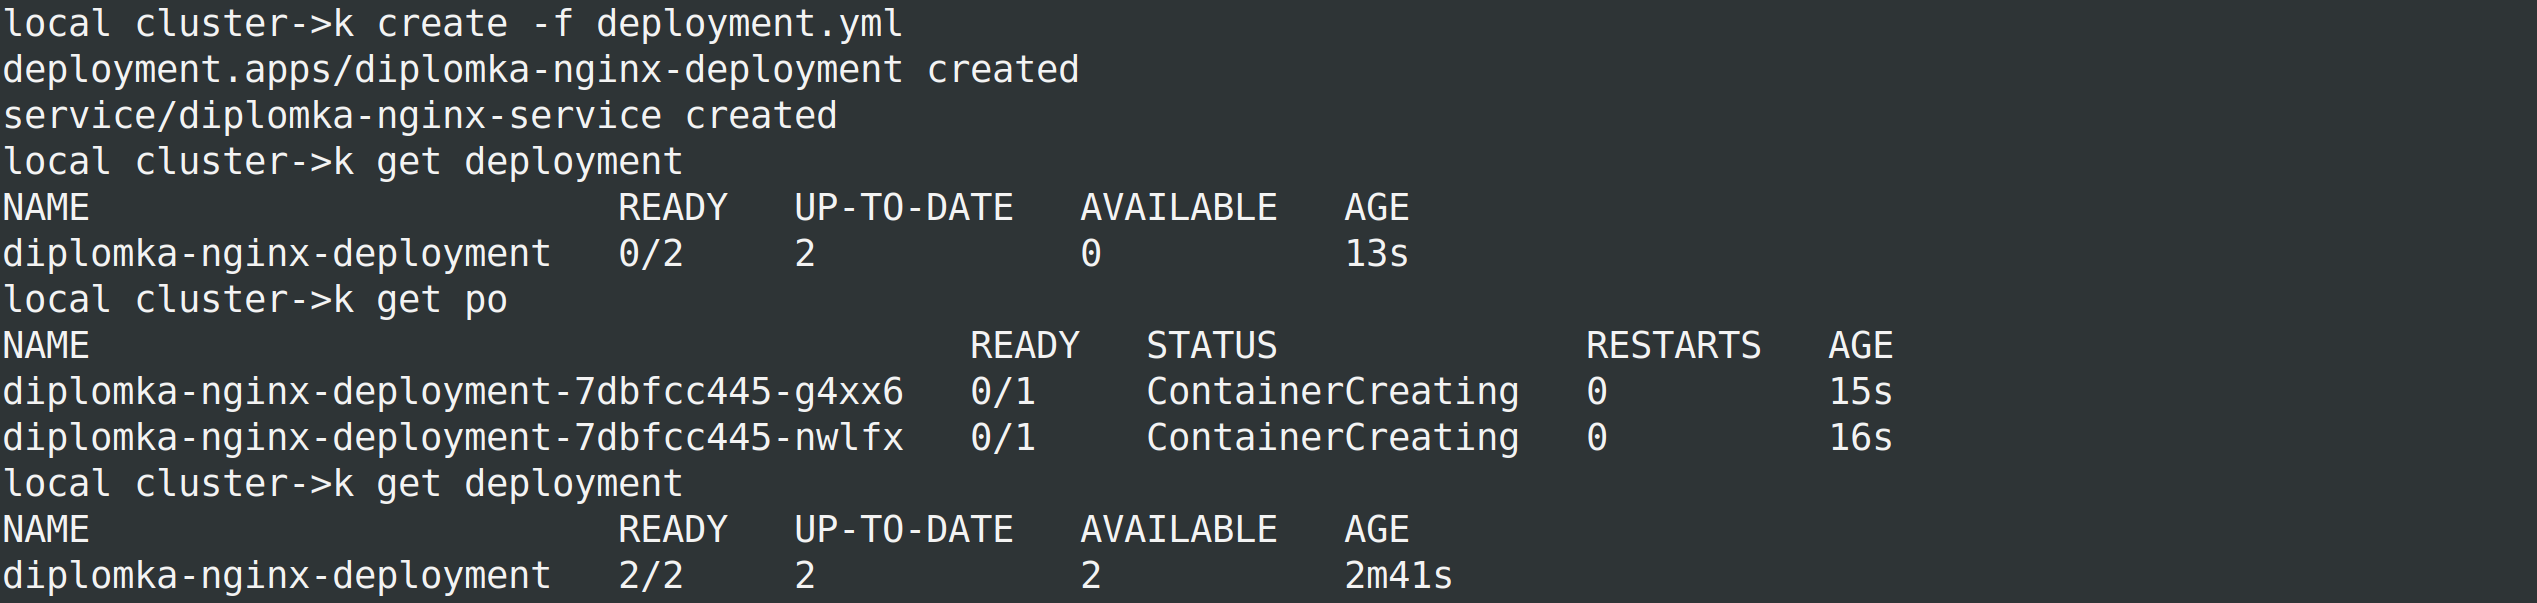
\includegraphics[width=0.9\textwidth]{images/create-deployment.png}
    \par
	  \caption{Vytvoření deploymentu\label{fig:create-deployment}, zdroj: vlastní tvorba}
    \end{centering}
\end{figure}

Výsledná aplikace je zobrazena na obrázku \ref{fig:v1}. Aplikace je dostupná na portu, který minikube cluster alokoval. V definici deploymentu byla specifikována verze 1, která koresponduje s hlavním titulkem na obrázku \ref{fig:v1}.

\begin{figure}[H]
  \begin{centering}
    
	  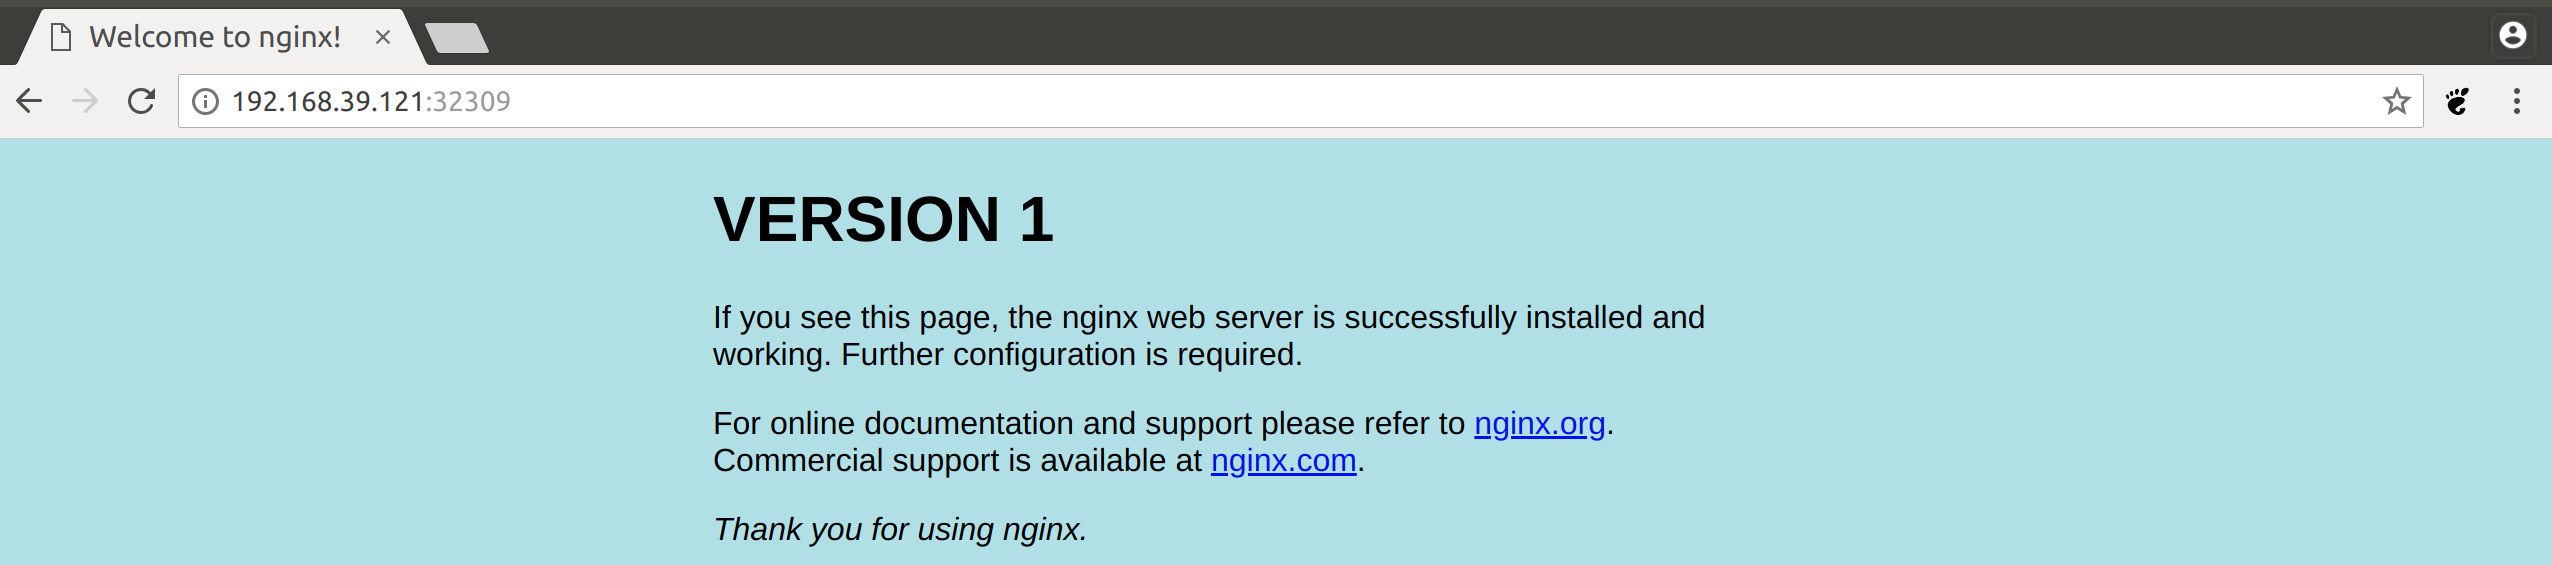
\includegraphics[width=0.9\textwidth]{images/v1.png}
    \par
	  \caption{Vzhled aplikace verze 1\label{fig:v1}, zdroj: vlastní tvorba}
    \end{centering}
\end{figure}

Jedním z rysů a výhod cloud native přístupu je doručování nových verzí aplikace. Cloud native aplikace nejsou statické co se týče nových funkcí a vylepšení. K8s dovoluje snadné nahrazení stávající verze novou verzí. V následujícím příkladu bude aplikace s verzí 1 nahrazena verzí aplikace 2. Postup přepnutí verze aplikace na verzi 2 je uveden na obrázku \ref{fig:update-deployment}. Na prvním řádku je zobrazena verze aplikace před upgradem. Na druhém řádku je pomocí příkazu edit uvedena změněna verze v definici deploymentu, která je následně zobrazena. V tomto okamžiku již k8s provádí vypnutí kontejnerů verze 1 a začíná s postupným startováním kontejnerů s verzí 2. Aplikace s novou verzí je zobrazena obrázku \ref{fig:v2}, aplikace je dostupná na stejné adrese a portu.

\begin{figure}[H]
  \begin{centering}
    
	  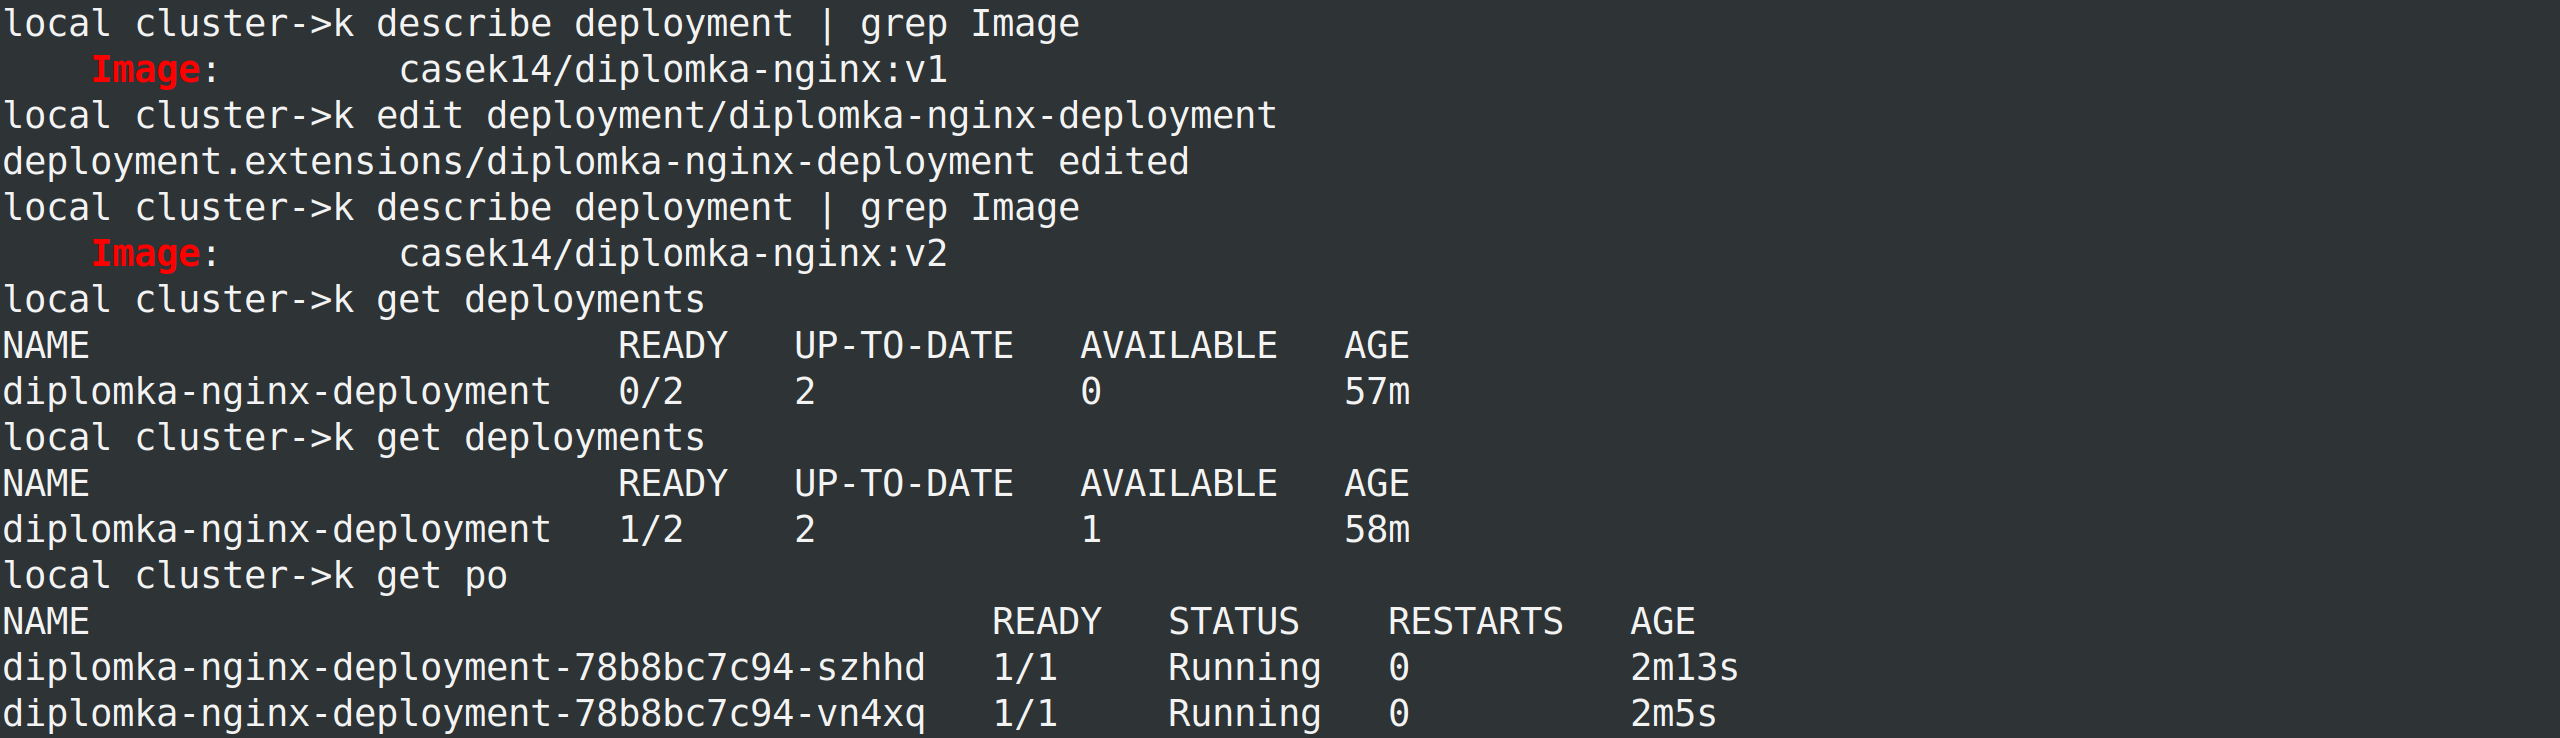
\includegraphics[width=0.9\textwidth]{images/deployment-update.png}
    \par
	  \caption{Úprava deploymentu\label{fig:update-deployment}, zdroj: vlastní tvorba}
    \end{centering}
\end{figure}

\begin{figure}[H]
  \begin{centering}
    
	  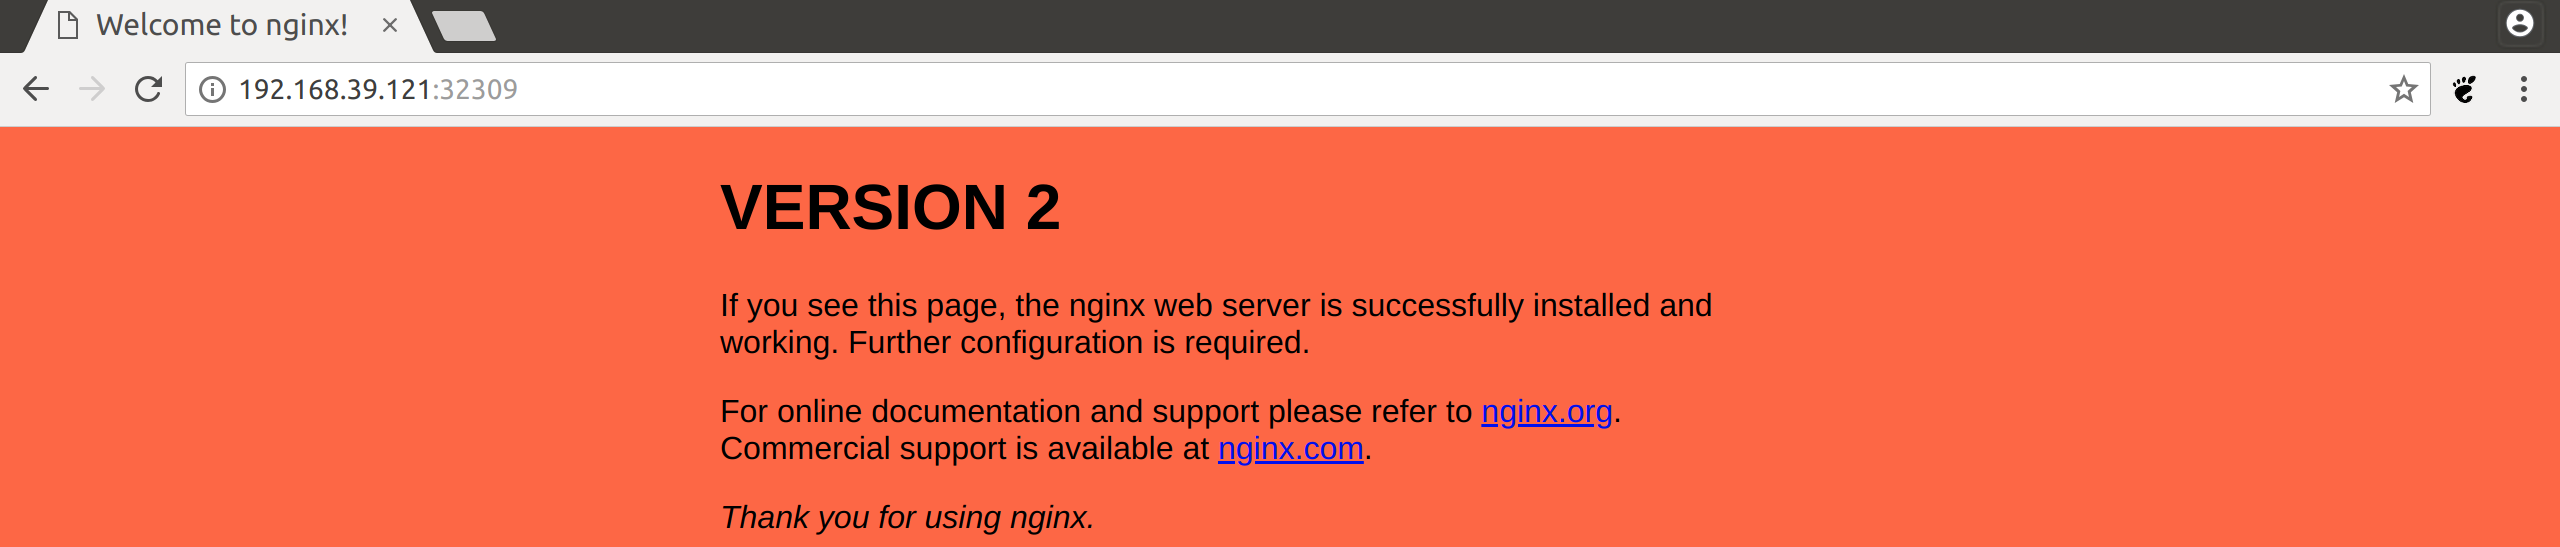
\includegraphics[width=0.9\textwidth]{images/v2.png}
    \par
	  \caption{Vzhled apliakce verze 2\label{fig:v2}, zdroj: vlastní tvorba}
    \end{centering}
\end{figure}
Deployment může být použitý také pro vrácení chybné verze aplikace. Tato technika je užitečná v okamžiku, že se do produkčního prostředí dostane verze aplikace, která nefunguje nebo obsahuje bug. Při testování této funkce, které je zobrazeno na obrázku \ref{fig:deployment-rollout}, je nejdříve vytvořen deployment s aplikací verze 1. Následně byla verze aplikace změněna na verzi 2, tato akce byla uložena pomocí volby “--record”. K8s si tuto akci uloží, aby bylo možné se vrátit o krok zpět. Následně je změněna verze aplikace na v3. Třetí verze aplikace je zobrazena na obrázku \ref{fig:v3}. Po nasazení třetí verze je ovšem zjištěno, že barva pozadí aplikace neodpovídá zadání. Zřejmě došlo k pochybení programátora, a barva pozadí neodpovídá barvám, které společnost využívá. Proto je rozhodnuto vrátit aplikaci do verze 2. K tomuto účelu byla využita funkce “rollout”, která vrátí verzi aplikace o jeden krok zpět na požadovanou verzi 2.

\begin{figure}[H]
  \begin{centering}
    
	  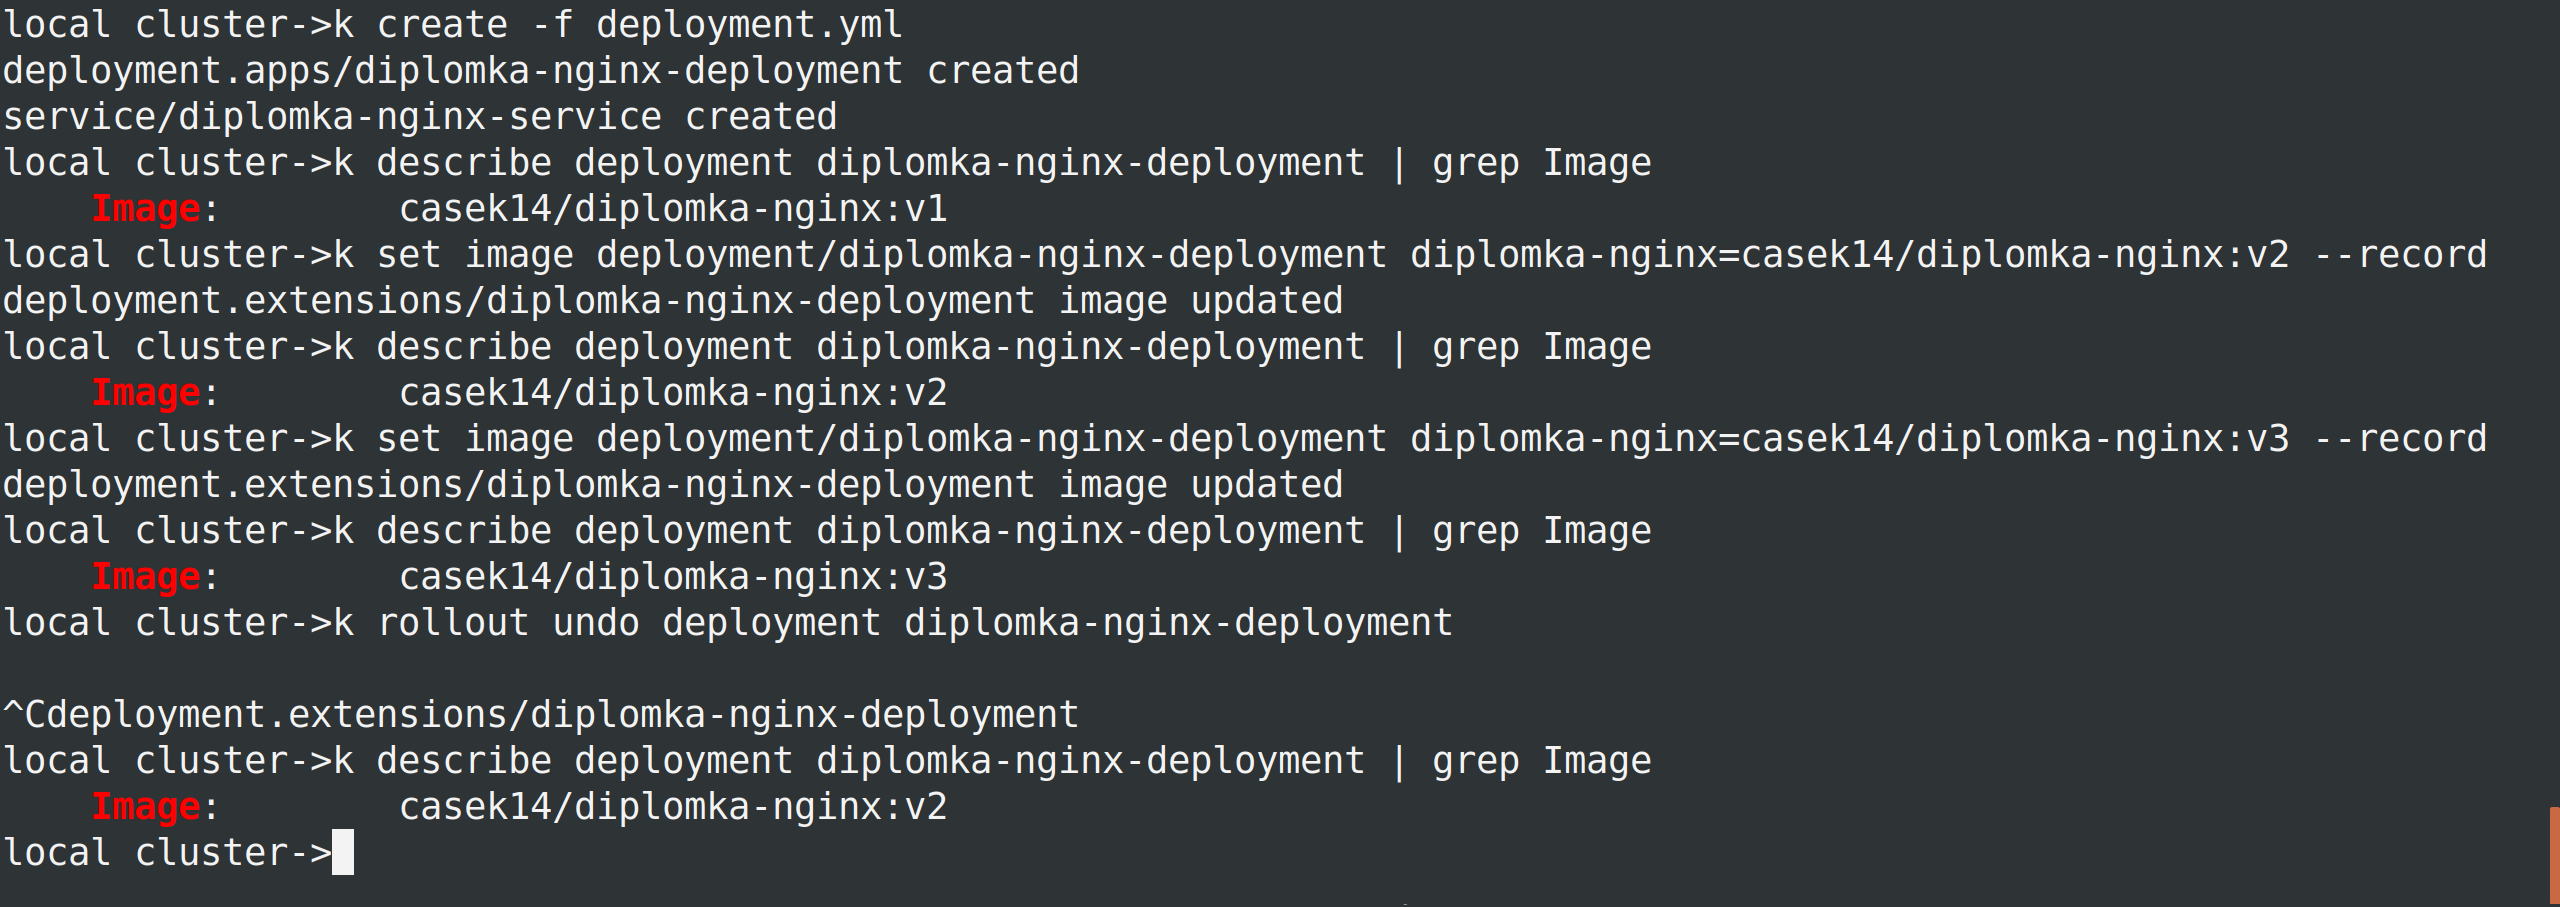
\includegraphics[width=0.9\textwidth]{images/rollout.png}
    \par
	  \caption{Vrácení verze aplikace pomocí rollout funkce\label{fig:deployment-rollout}, zdroj: vlastní tvorba}
    \end{centering}
\end{figure}

\begin{figure}[H]
  \begin{centering}
    
	  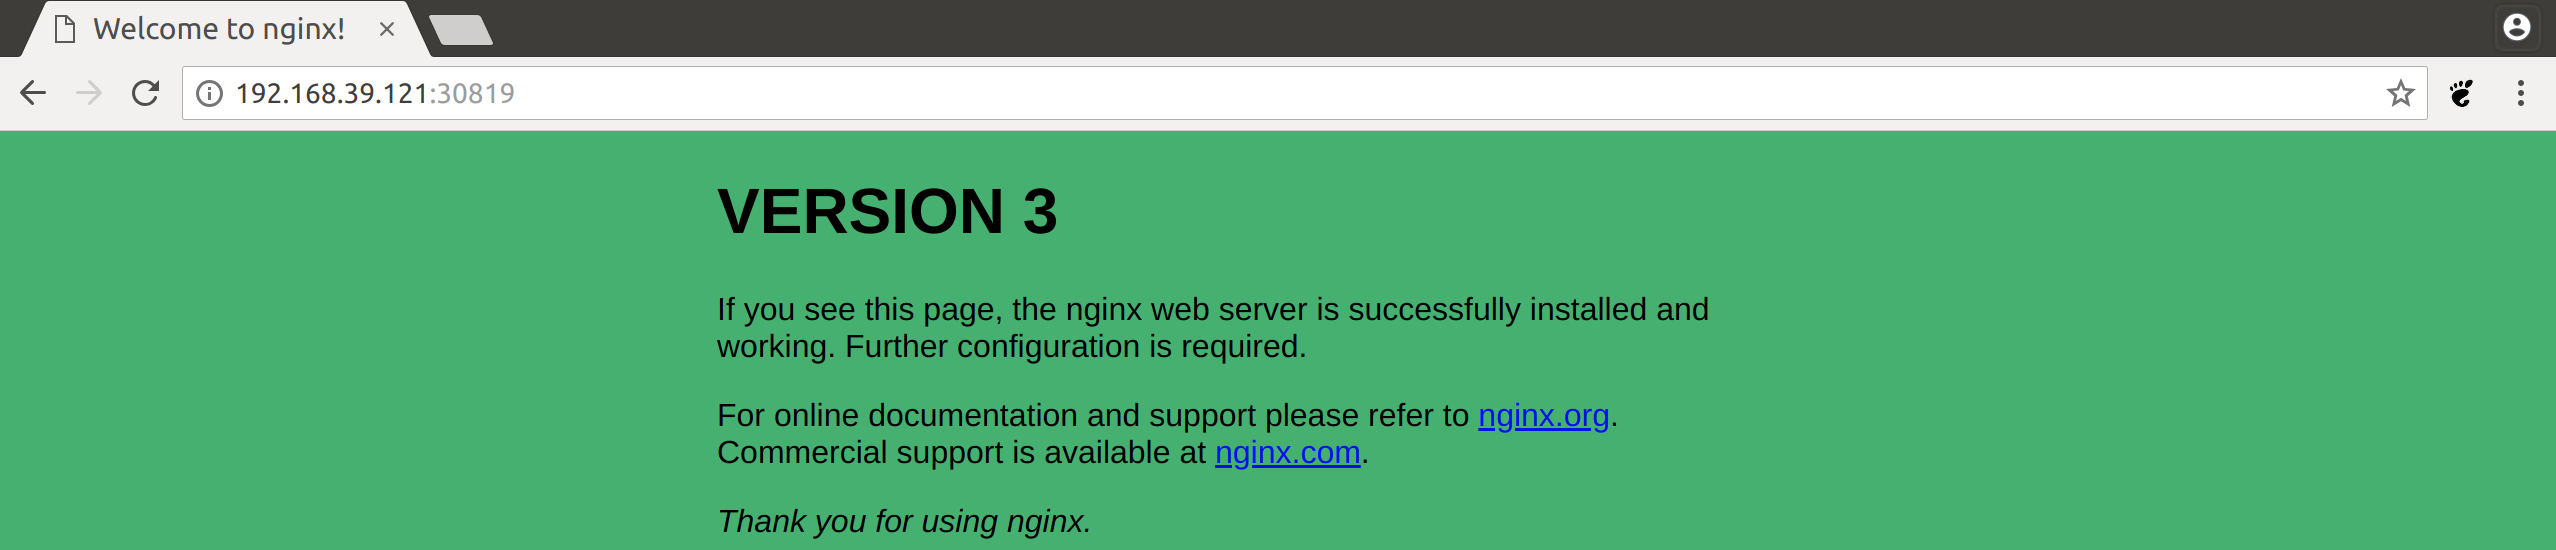
\includegraphics[width=0.9\textwidth]{images/v3.png}
    \par
	  \caption{Vzhled aplikace verze 3\label{fig:v3}, zdroj: vlastní tvorba}
    \end{centering}
\end{figure}

Jedním z testovaných aspektů je i škálování aplikací. Pokud současný počet instancí aplikace nestíhá obsloužit všechny zákazníky je potřeba zvýšit jejich počet. K8s opět nabízí pro tento účel nástroje, které dovolují operátorům jednoduše zvýšit počet instancí. Service se postará o rozložení zátěže mezi všechny nové pody. Na obrázku \ref{fig:scale1} je vytvořen deployment, který se skládá ze dvou podů a také service směřující požadavky na tyto pody. Každý pod na portu 80 odpovídá na požadavky se svým jménem kontejneru. Zdrojový kód této aplikace je uveden v příloze \hyperref[app:hostname]{A}. Dále je spuštěn skript, který desetkrát pošle požadavek na service a vypíše odpověď. Z obrázku je patrné, že požadavky vyřizují pouze dva pody.

\begin{figure}[H]
  \begin{centering}
    
	  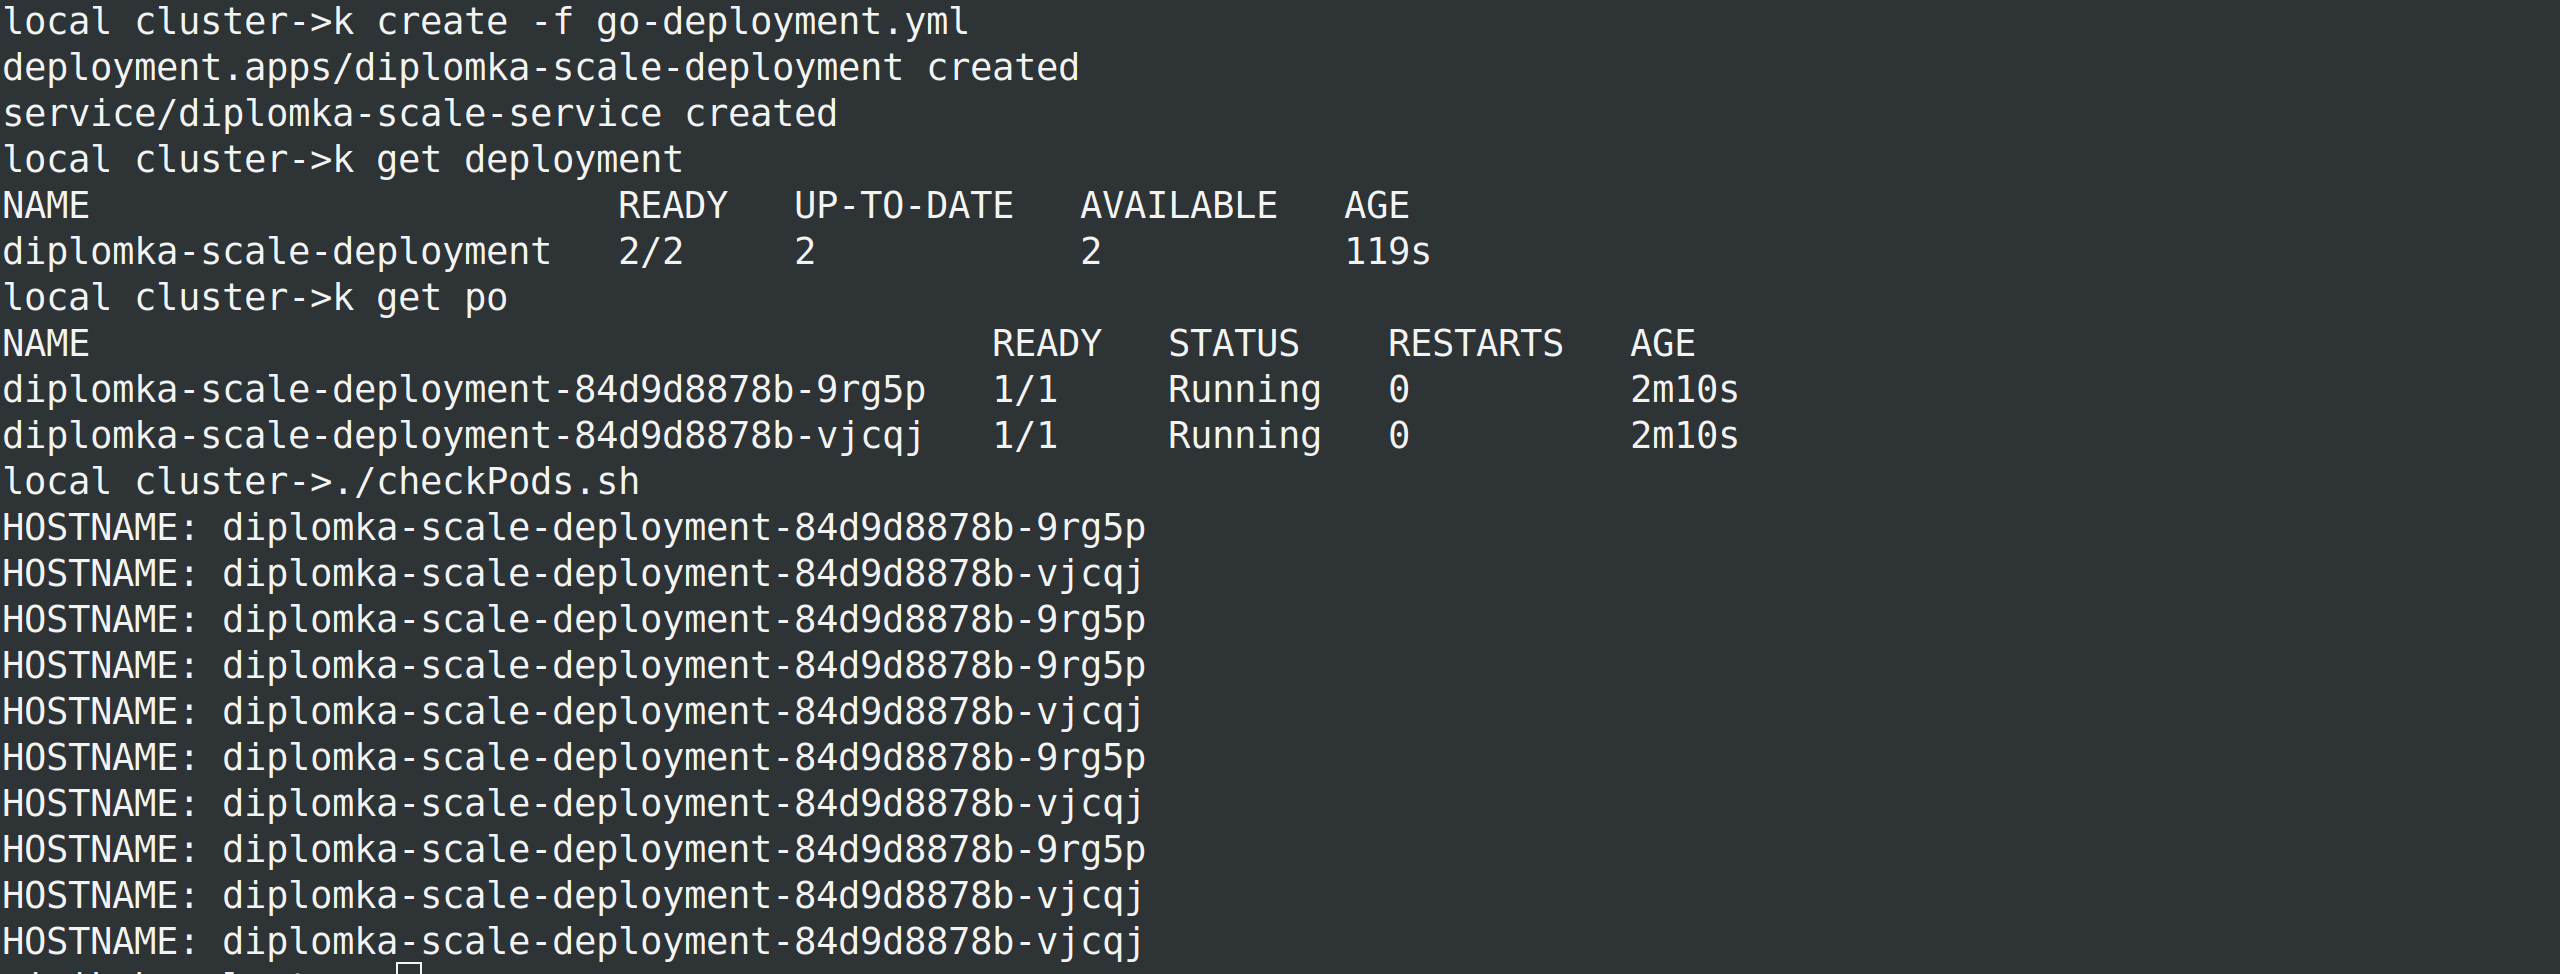
\includegraphics[width=0.9\textwidth]{images/scale1.png}
    \par
	  \caption{Test deploymentu se 2 pody\label{fig:scale1}, zdroj: vlastní tvorba}
    \end{centering}
\end{figure}

V dalším kroku je počet podů, které budou vyřizovat požadavky uživatelů zvýšen na deset \ref{fig:scale2}. K8s ihned začne startovat nové kontejnery tak, aby bylo dosaženo \linebreak požadovaného počtu deseti instancí aplikace. V přehledu podů je vidět, že dva původní pody zůstaly a k nim byly vytvořeny další pody. Patrné je to podle parametru “AGE” neboli stáří kontejneru.

\begin{figure}[H]
  \begin{centering}
    
	  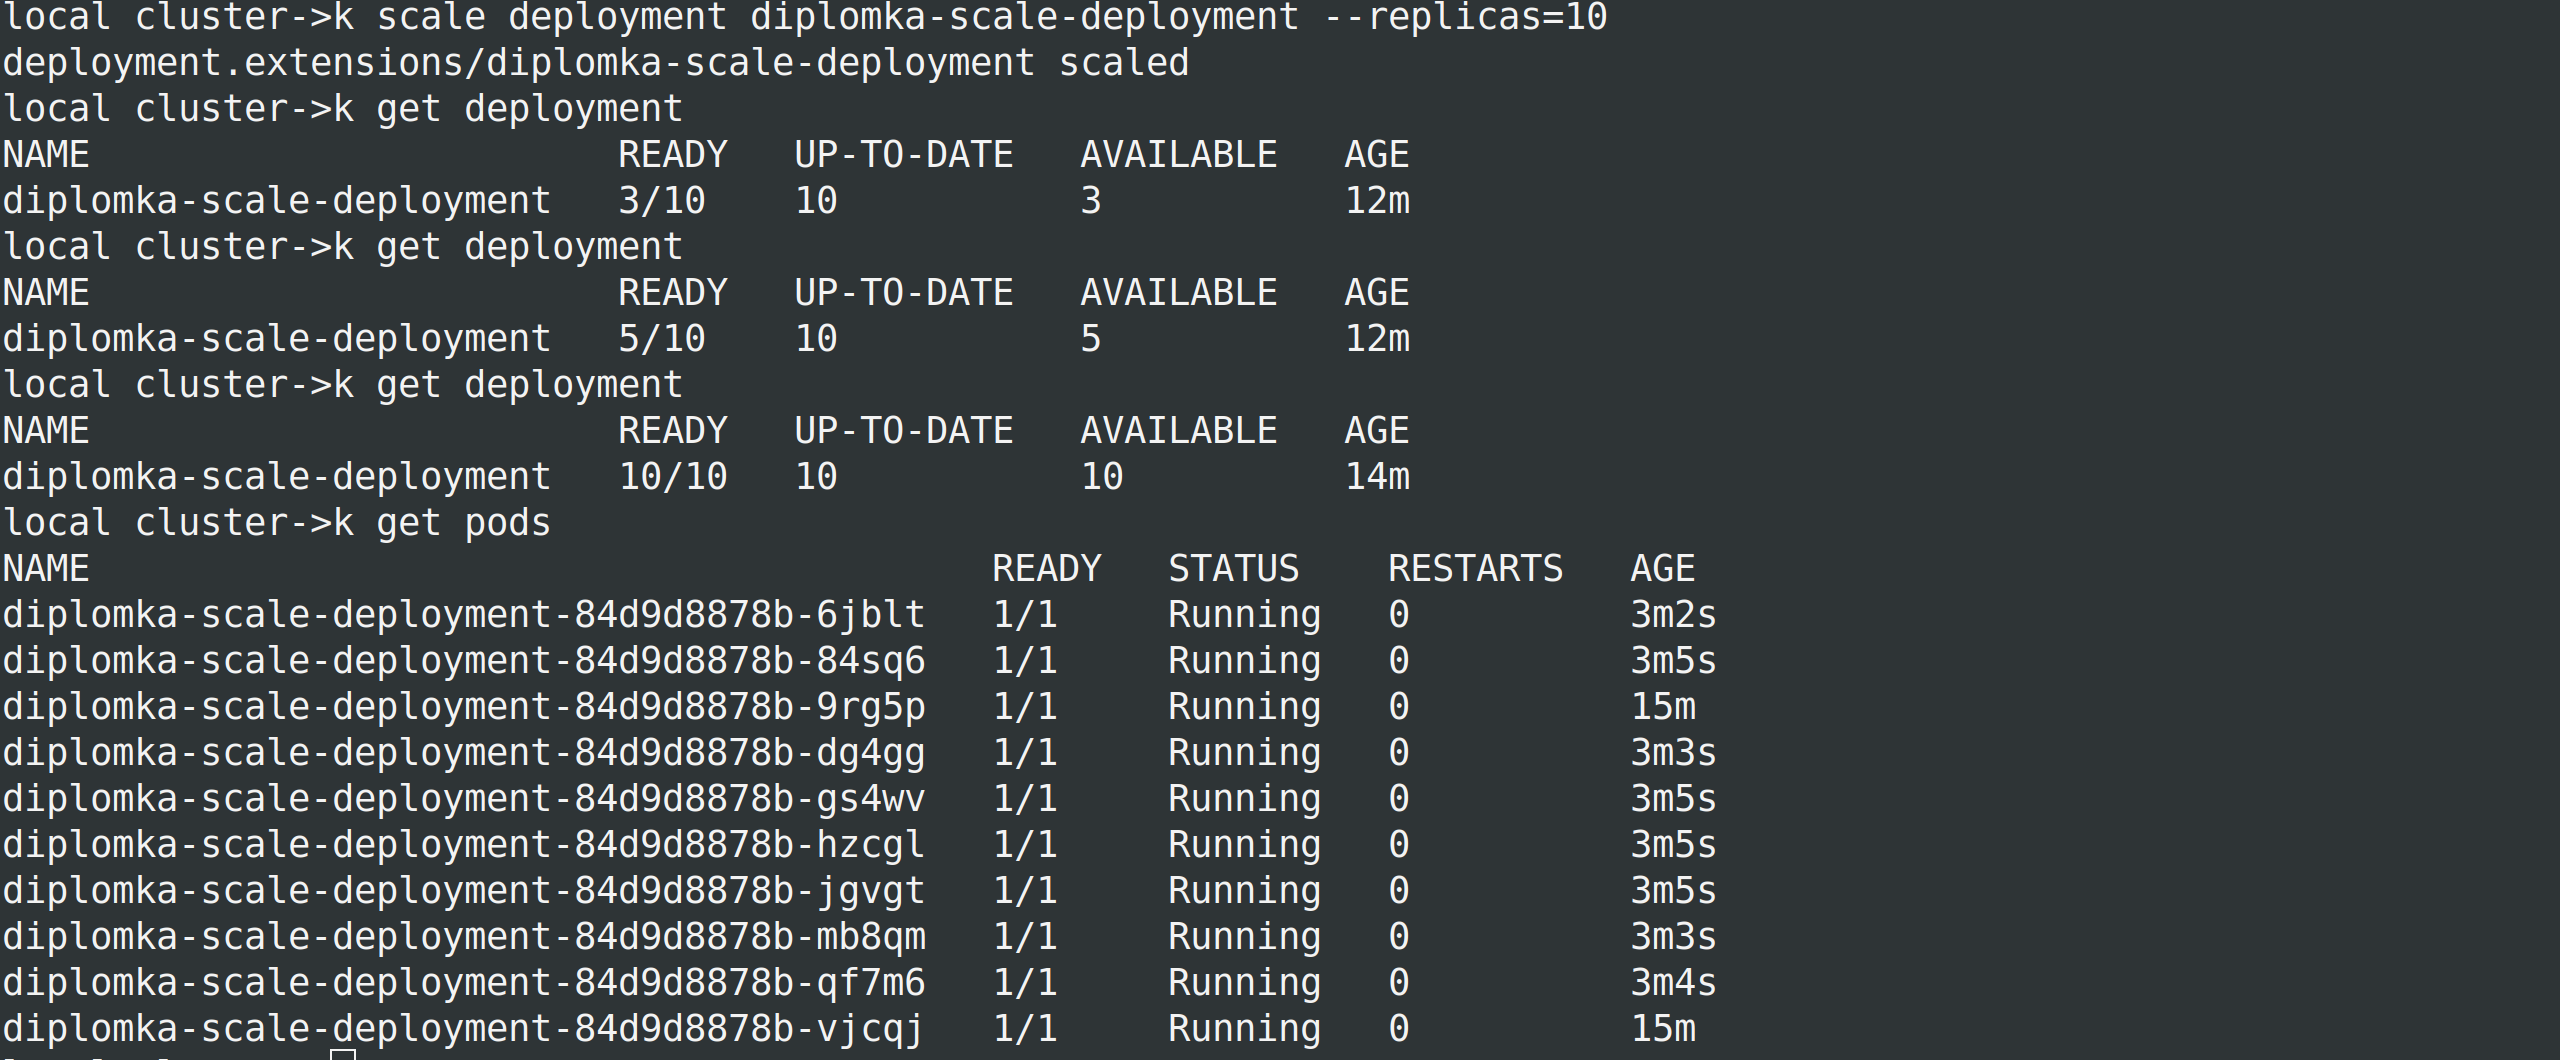
\includegraphics[width=0.9\textwidth]{images/scale2.png}
    \par
	  \caption{Škálování deploymentu ze 2 na 10 podů\label{fig:scale2}, zdroj: vlastní tvorba}
    \end{centering}
\end{figure}

Servica, která se stará o rozdělení zátěže, směřuje požadavky i na nově vytvořené pody, které vybírá podle labelu app=golang. Na obrázku \ref{fig:scale3} je zobrazen výstup ze skriptu, požadavky směřují pokaždé na jeden z deseti podů, které obsahují aplikaci.

\begin{figure}[H]
  \begin{centering}
    
	  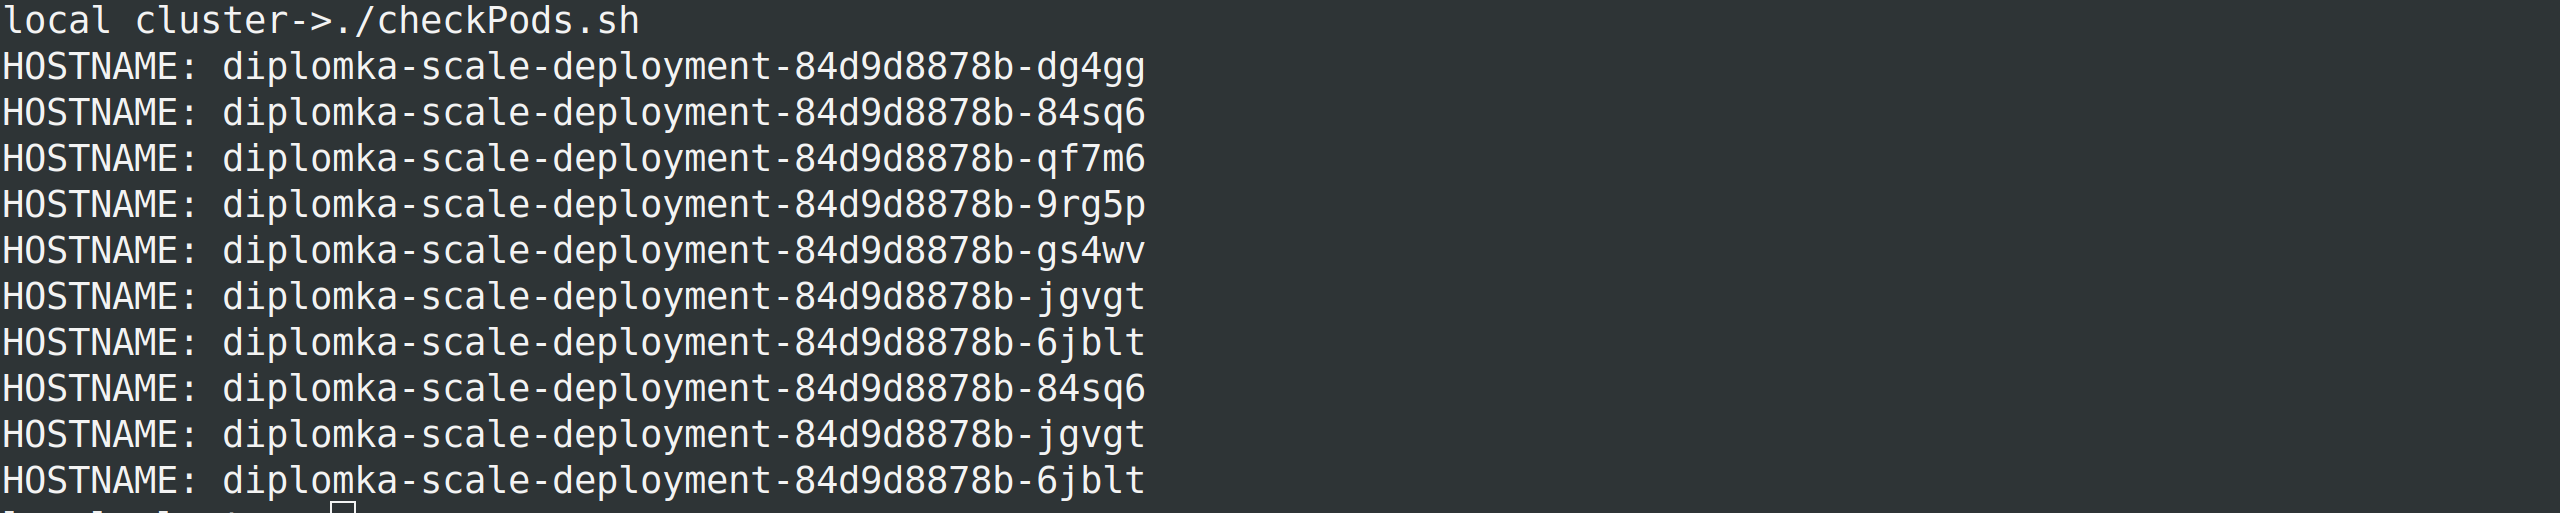
\includegraphics[width=0.9\textwidth]{images/scale3.png}
    \par
	  \caption{Test dostupnosti deploymentu s 10 pody\label{fig:scale3},  zdroj: vlastní tvorba}
    \end{centering}
\end{figure}

\subsection{Distribuce Kubernetes statefulset objektů}
Kubernetes umožňuje běh stateful aplikací, které uchovávají a spravují data. Příkladem stateful aplikací jsou databáze. Databáze potřebují uložiště pro data, které vydrží restart kontejnerů. Tato funkcionalita je v k8s reprezentována pomocí zdroje statefulset. Statefulset je obdobou deploymentu, ale pro stateful aplikace. Statefulset řídí počet replik, jejíž pody jsou vytvářeny jeden po druhém, mají definované pořadí a přiřazené stejné uložiště. Pokud statefulset obsahuje tři repliky, jako první se vytvoří replika jedna a až po jejím úspěšném vytvoření a spuštění se začne spouštět druhá replika a poté následuje třetí replika. Uložiště je do podu připojeno jako volume. Ovšem statefulset po restartování kontejneru tento volume nesmaže a tak nedojde ke ztrátě dat. Pro vytvoření volumu jsou použity tři k8s zdroje storageclass, persistenvolume (PV) a persistentvolumeclaim (PV). Storageclass představuje reprezentaci uložiště, kterou k8s cluster nabízí a obsahuje například parametr provisioner, který specifikuje jaký typ uložiště bude použitý. Může být použit NFS, CEPH a spoustu dalších. Příklad definice storage class je uveden v ukázce kódu \ref{lst:storageclass}. PV abstrahuje implementační detaily jednotlivých typů uložišť a je spravováno administrátorem k8s clusteru. PVC je požadavek uživatele pro přidělení uložiště pro určitý pod. PVC je alokováno z PV. 

\begin{lstlisting}[caption={StorageClass definice pro minikube cluster},label=lst:storageclass]
kind: StorageClass
apiVersion: storage.k8s.io/v1
metadata:
  name: minikube-class
  provisioner: k8s.io/minikube-hostpath
  reclaimPolicy: Retain
\end{lstlisting}

\par
      Pro otestování distribuce stateful aplikací je použita jednoduchá aplikace, která po svém spuštění vytvoří ve specifickém adresáři soubor, jehož jméno je složeno z hostnamu daného kontejneru a časového údaje, kdy byl vytvořen. Aplikace následně po vytvoření souboru zpřístupní tento adresář se souborem na portu 3000. Zdrojový kód aplikace je uveden v příloze \hyperref[app:servefiles]{B}. Pro spuštění této aplikace je použitý manifest soubor uvedený v příloze \hyperref[app:statefulset]{C}. Definice statefulsetu začíná definicí názvu této aplikace, následuje specifikace selektoru, tedy jaké pody patří k tomuto statefulsetu. Definice kontejneru a portu na kterém aplikace zpracovává požadavky je známá z předchozích příkladů. Definice “volumeMounts” reprezentuje trvalé uložiště, které bude připojené ke kontejneru a do něhož bude aplikace ukládat zmíněné soubory. Definice samotného uložiště je uvedena pod částí “volumeClaimTemplates”, která říká jaké uložiště bude použito. Parametr “storageClassName” se shoduje s názvem v definici pro strorageclass \ref{lst:storageclass}. Velikost uložiště, které bude připojené k podu připojené má velikost 1GB. Poslední částí definice statefulsetu je definice systémové proměné “DIRECTORY\_PATH”, kterou aplikace využívá pro nastavení adresáře, kam jsou ukládány soubory, jejichž výpis je dostupný na portu 3000 daného podu. Tato systémová proměnná je definovaná s využitím dalšího k8s zdroje secretu. Secret slouží k uložení a správě citlivých informací jako jsou hesla, tokeny nebo ssh klíče. Definice secretu obsahuje název daného secretu, na který se poté odkazujeme v definici systémové proměnné v definici podu. Secret dále obsahuje data, která jsou použita pro nastavení hodnoty systémové proměnné. Hodnota je uložena jako klíč a k němu odpovídající hodnota. Aby nebyla cesta k adresáři se soubory uvedena pouze jako text, byla ještě zakódovaná pomocí nástroje base64 \ref{lst:base}. Výsledkdem je hash, který reprezentuje cestu k adresáři. Tato cesta je shodná s cestou do které je připojené uložiště pro aplikaci, konkrétně je to adresář “/diplomka-serve-files”.

\begin{lstlisting}[caption={Zakódování textu pomocí base64 nástroje},label=lst:base]
      local cluster->echo -n '/diplomka-serve-files' | base64
      L2RpcGxvbWthLXNlcnZlLWZpbGVz
      local cluster->echo 'L2RpcGxvbWthLXNlcnZlLWZpbGVz' | base64 --decode
      /diplomka-serve-files
\end{lstlisting}

\par      Proces práce s statefulset aplikací je zobrazen na obrázku \ref{fig:statefulset}. Nejdříve jsou \linebreak vytvořeny všechny potřebné zdroje, secret, statefulset a nakonec servica, která aplikaci zpřístupní uživatelům. Po stažení imagů jsou kontejnery v podu spuštěny. Ve výpisu podů je vidět, že druhý kontejner byl spuštěn pět vteřin po prvním kontejneru, to je vlastnost statefulsetu, který spouští kontejnery jeden po druhém na rozdíl od deploymentů, kde jsou všechny pody spuštěny současně. Obrázek \ref{fig:curl1} zobrazuje stav oboud podů. Každý pod obsahuje právě jeden soubor, protože byly spuštěny pouze jednou. V další kroku dojde k okamžitému smazání podu fileserver-0. Tato akce donutí statefulset k vytvoření nového podu s aplikací. Ačkoliv se bude jednat o jiný pod, jeho název bude stejný a stejně tak mu budou připojena již existující data vytvořená existujícím podem. Na obrázku \ref{fig:statefulset} ve výpisu podů po smazání jednoho z nich je patrné, že nově vytvořený pod běží pouhé dvě minuty, kdežto druhý pod fileserver-1 běží od počátku bez restartu již minut šest. Obrázek \ref{fig:curl2} zobrazuje výpis dat. Pod fileserver-1 obsahuje pouze jeden soubor a pod fileserver-0 obsahuje právě dva soubory. Statefulset zdroj tedy aplikace byla aplikace schopná obsloužit, data se uchovala i mezi restartem podů.

\begin{figure}[H]
  \begin{centering}
	  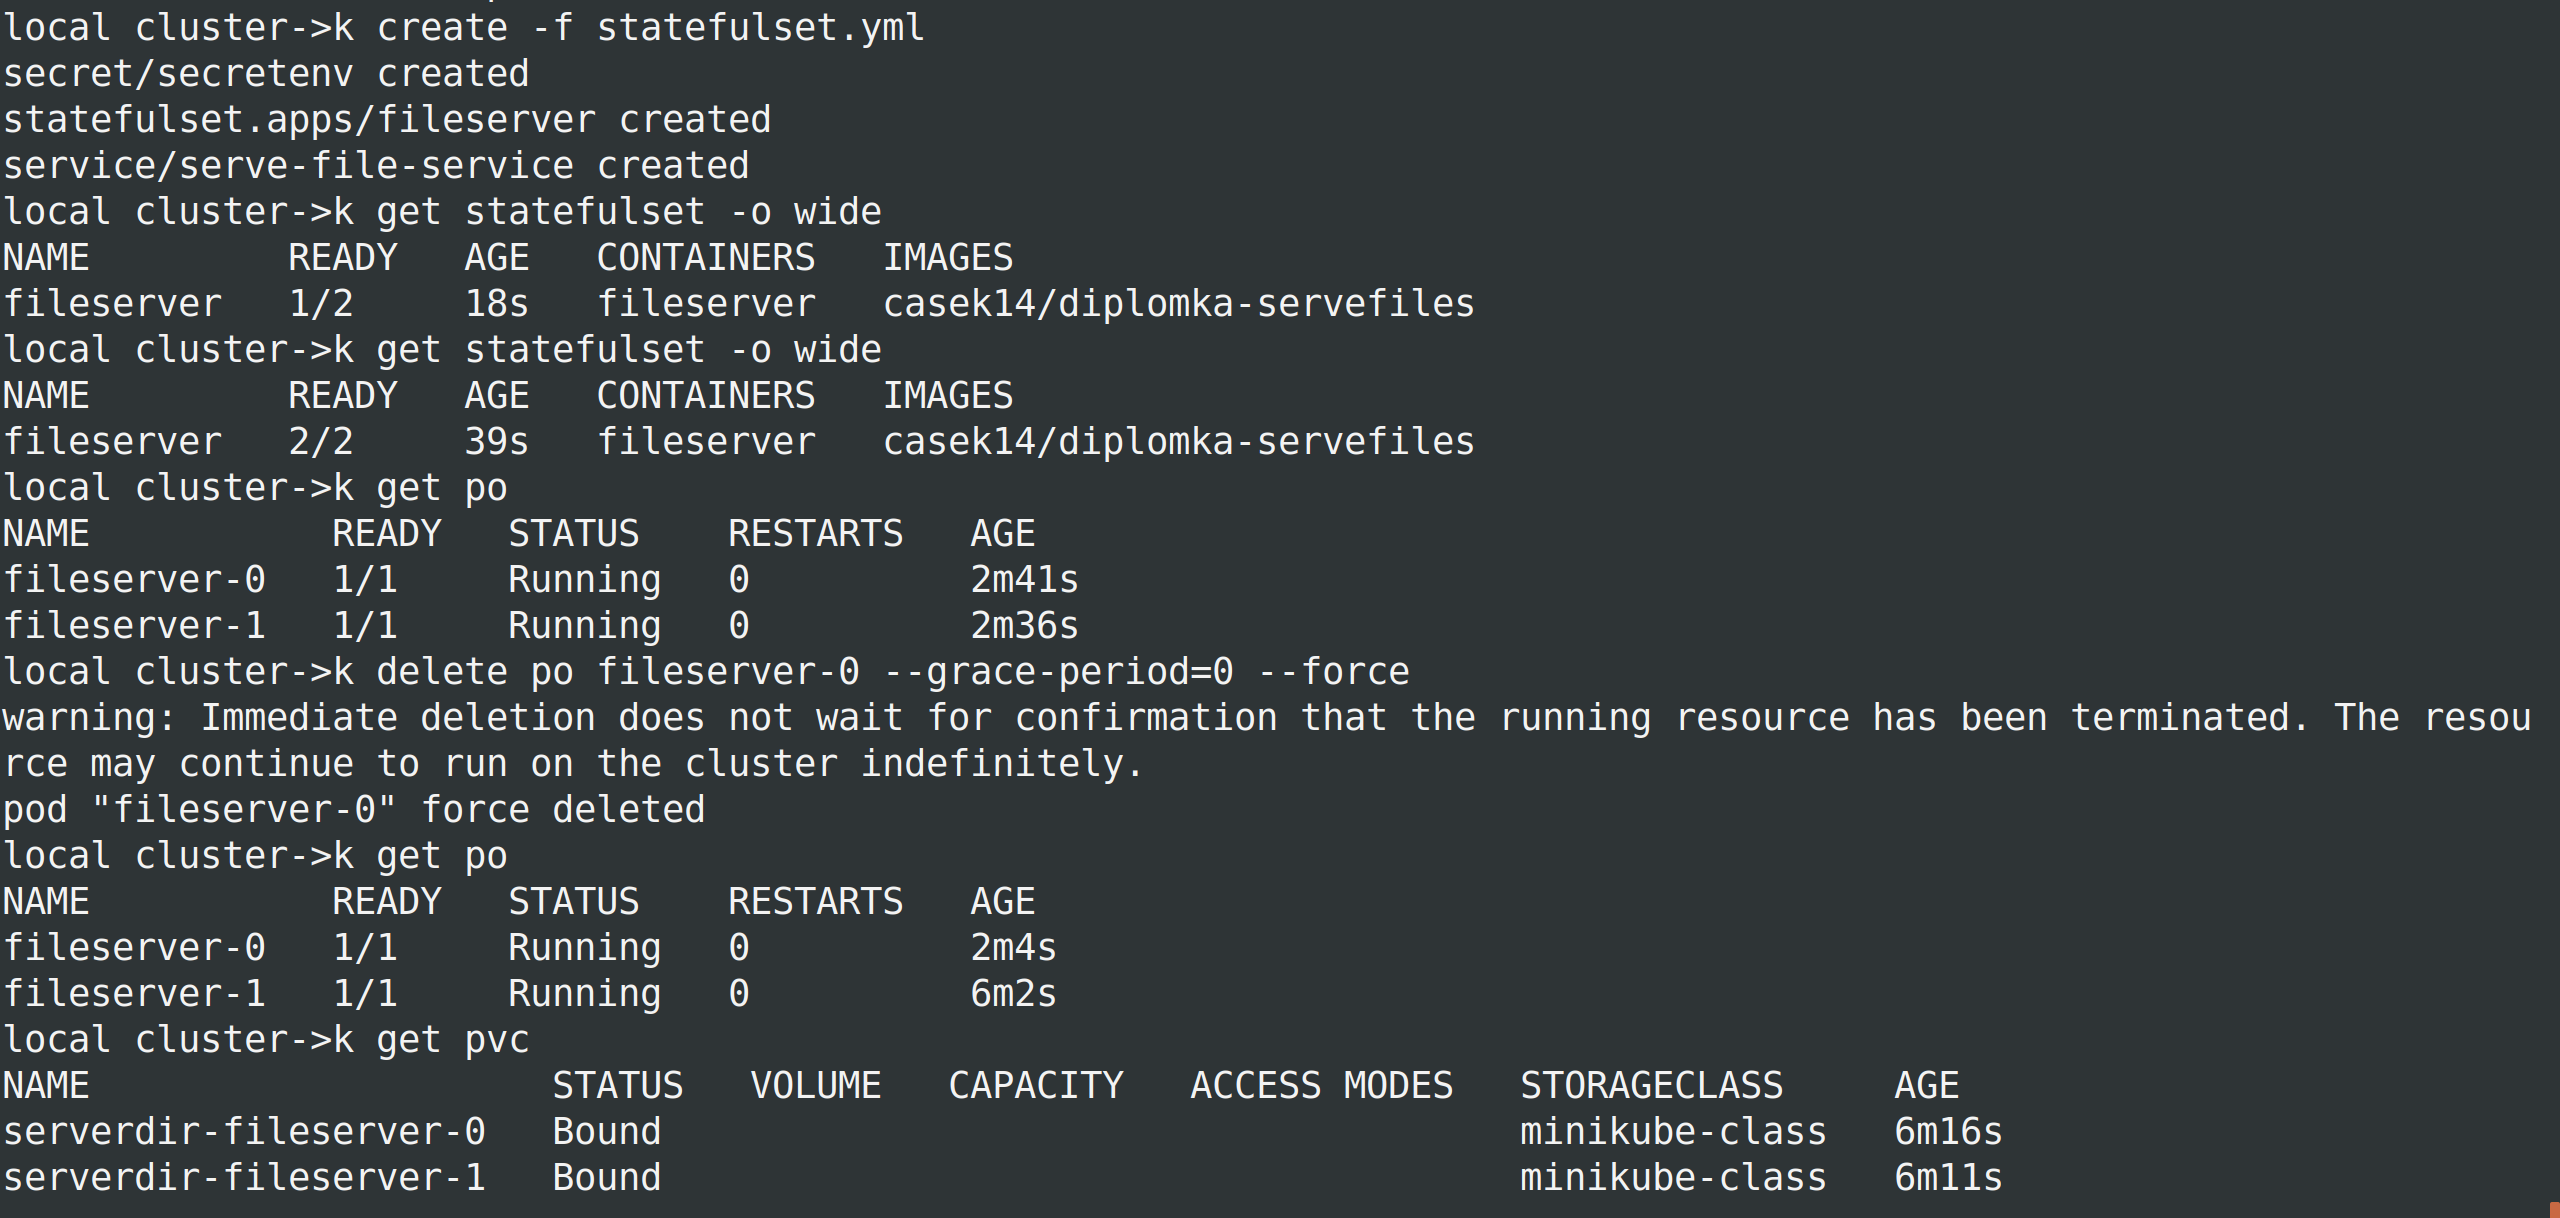
\includegraphics[width=0.9\textwidth]{images/statefulset.png}
    \par
	  \caption{Vytvoření a otestování statefulsetu\label{fig:statefulset}, zdroj: vlastní tvorba}
    \end{centering}
\end{figure}


\begin{figure}[H]
  \begin{centering}
	  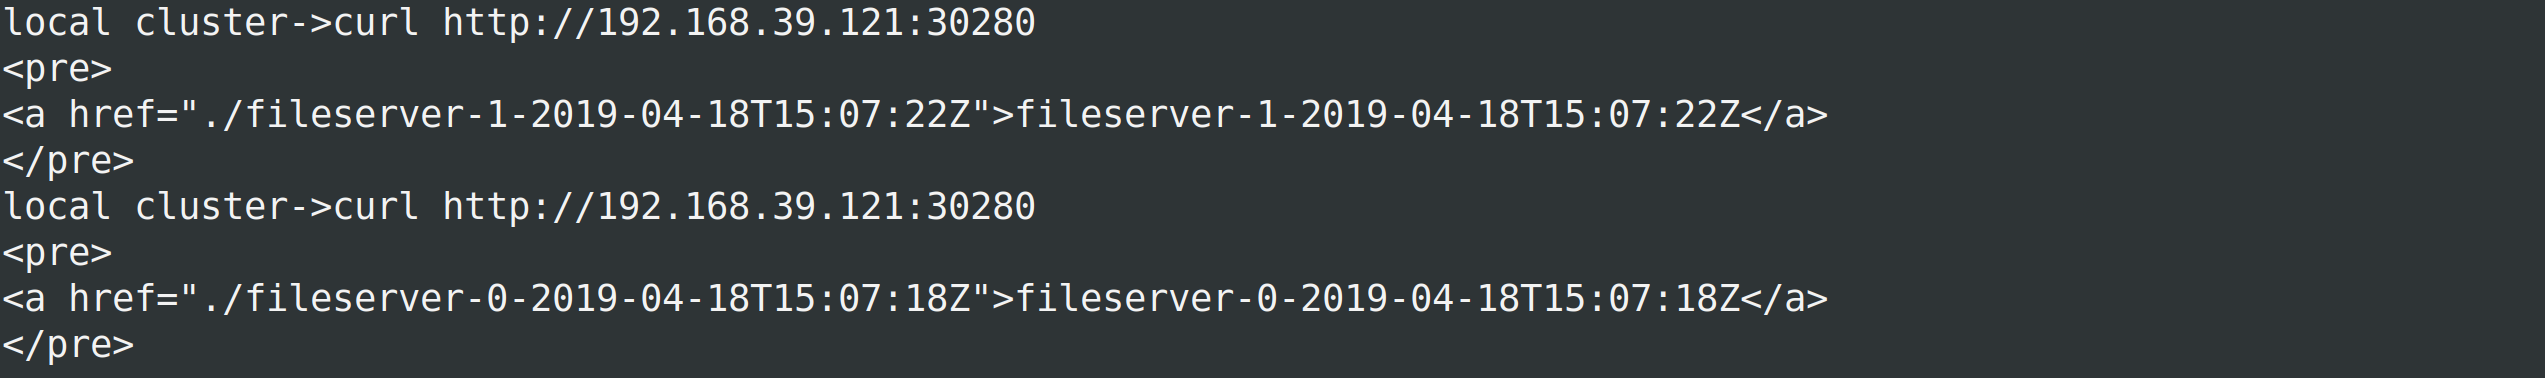
\includegraphics[width=0.9\textwidth]{images/curl1.png}
    \par
	  \caption{Data statelful aplikace\label{fig:curl1}, zdroj: vlastní tvorba}
    \end{centering}
\end{figure}

\begin{figure}[H]
  \begin{centering}
	  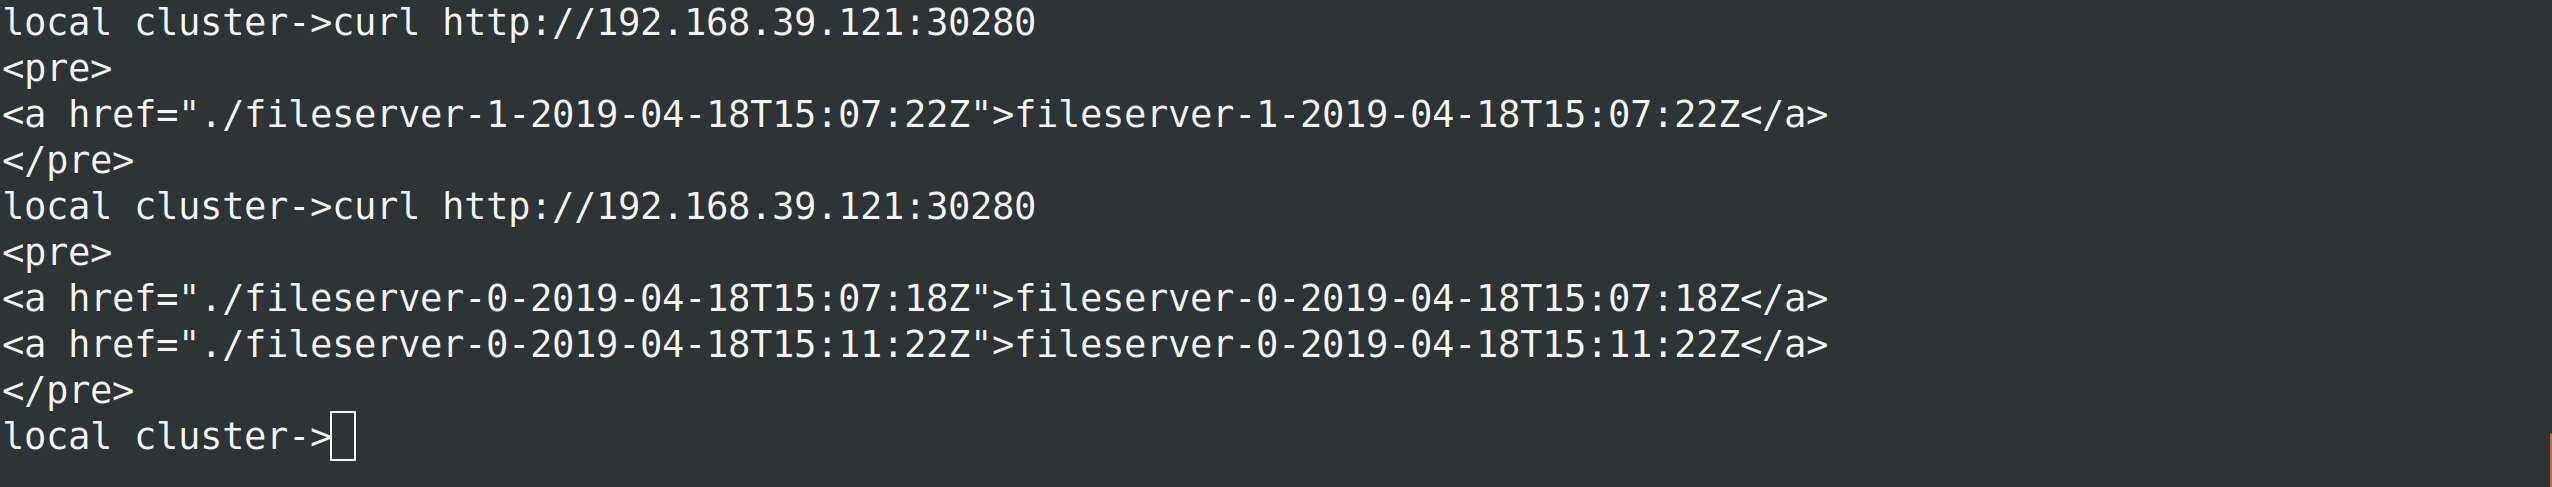
\includegraphics[width=0.9\textwidth]{images/curl2.png}
    \par
	  \caption{Data stateful aplikace po restartu jednoho z podů\label{fig:curl2}, zdroj: vlastní tvorba}
    \end{centering}
\end{figure}
